\documentclass[11pt]{article}

\usepackage[margin=1in]{geometry}
\usepackage[T1]{fontenc}
\usepackage[utf8]{inputenc}
\usepackage{lmodern}
\usepackage{amsmath,amssymb,amsfonts}
\usepackage{xcolor}
\usepackage[hidelinks,pdftitle={LUTGPT: a rank-mediated transformer backbone via differentiable lookup tables}]{hyperref}
\usepackage{xurl}
\usepackage{enumitem}
\usepackage{titlesec}
\usepackage{booktabs}
\usepackage{array}
\usepackage{verbatim}
\usepackage[numbers]{natbib}
\usepackage{tikz}
\usetikzlibrary{positioning, arrows.meta, fit, calc, shapes.geometric}
\usepackage{placeins}

\setlength{\parskip}{2pt}
\titlespacing*{\section}{0pt}{10pt plus 2pt minus 2pt}{4pt}
\titlespacing*{\subsection}{0pt}{8pt plus 2pt minus 2pt}{3pt}
\titlespacing*{\paragraph}{0pt}{4pt plus 1pt minus 1pt}{6pt}

\newcommand{\R}{\mathbb{R}}
\newcommand{\sign}{\mathrm{sign}}
\newcommand{\softmax}{\mathrm{softmax}}
\newcommand{\Tsel}{T_{\mathrm{sel}}}
\newcommand{\Tsoft}{T_{\mathrm{soft}}}
\newcommand{\dqk}{d_{qk}}
\newcommand{\dv}{d_v}
\newcommand{\dout}{D_{\mathrm{out}}}
\newcommand{\bstar}{b^{\star}}
\newcommand{\jstar}{j^{\star}}

\title{\Large\textbf{LUTGPT: a rank-mediated transformer backbone via differentiable lookup tables}\\[3pt]
\large An existence proof at nanochat scale, a transparent efficiency profile, and a hardware bet}
\author{Anatoly Starostin \and Eugene Izhikevich}
\date{}

\begin{document}
\maketitle
\vspace{-12pt}

% =========================================================================
\begin{abstract}
\noindent
We start from a working hypothesis that the computation performed inside a spiking neural network can be modelled, in the abstract, as a sequence of mappings between rank/order patterns of input activations and rank/order patterns of output activations~\citep{manifesto}. A differentiable lookup-table (LUT) primitive is the natural carrier of such mappings: each table decodes its input by pairwise sign comparisons of selected anchor pairs, emits a learnt row, and trains via a soft surrogate of that discrete decision. A toy LUT transformer was proposed earlier as a proof-of-concept but never tested on real text at real context length and a real vocabulary size.

This report asks whether the LUT family can extend to a model that works at nanochat scale~\citep{karpathy_nanochat}: real ClimbMix text data, a real BPE tokeniser, real context length, and a real vocabulary size. We answer in the affirmative for the \emph{backbone}: the publishable model, LUTGPT, replaces every Q, K, V, output, and residual projection in a six-layer transformer with a multi-head LUT, and matches a vanilla baseline in validation loss at a matched training-token budget on the same data. Two interfaces remain Euclidean and require dense matrix multiplications --- scaled-dot-product attention (SDPA) and the linear unembedder; both are open problems we deliberately do not solve here. On current GPU hardware the LUT model is not competitive in wall-clock; we are explicit about this. The bet is on rank-coded sparse-lookup hardware that does not yet exist, for which the LUT family's $\sim$3--4$\times$ lower per-token HBM read on the backbone and bounded active-parameter set would become a decisive advantage.
\end{abstract}

\vspace{6pt}

% =========================================================================
\section{Introduction}

\subsection{The starting hypothesis}

The spiking manifesto~\citep{manifesto} sets out a working hypothesis: a spiking neural network, viewed as a computation, is a \emph{permutation mapper}. Its inputs are rank/order patterns over spike arrival times. Its outputs are new rank/order patterns over emitted spikes. What it computes is determined by the ordering of its inputs, not by their absolute magnitudes; how it does so --- the biophysics, the ion channels, the dendritic integration --- is an implementation detail.

Two consequences follow. First, the right abstraction for studying these networks is the mapping itself, not the dynamics. Second, that mapping is naturally captured by a finite, trainable, discrete object: a lookup table whose decision boundary is rank-coded and whose output rows are learnt by gradient descent on a soft surrogate. The manifesto proposes this LUT abstraction as the primitive of a new family of architectures and demonstrates a small proof-of-concept LUT transformer at short context. The demonstration shows the idea; it does not show whether the family scales.

\subsection{The LUT primitive in brief}
\label{ssec:lut-primer}

Here is a brief reminder of the LUT idea. The full derivation is in Section~\ref{sec:primitive}; here we only need a working picture.

A LUT layer maps an input vector $x$ to an output vector $y$ in two steps. \emph{(1) Encode by pairwise sign comparisons.} The layer fixes $N$ anchor pairs $(a_j, b_j)$ at initialisation. For each pair it computes one bit $\mathbf{1}[x_{a_j} > x_{b_j}]$, and packs the $N$ bits into a single row index
\[
b^\star \;=\; \sum_{j=1}^{N} \mathbf{1}[x_{a_j} > x_{b_j}] \cdot 2^{N-1-j} \;\in\; \{0, 1, \dots, 2^N - 1\}.
\]
The encoding is purely rank-coded: each bit depends only on the order of two coordinates of $x$, not on the magnitude of their difference. \emph{(2) Decode by row gather.} The layer holds a learned weight table $W \in \R^{2^N \times \dout}$ and outputs the gathered row $y = W[b^\star] \in \R^{\dout}$. The decoding is an arbitrary learned mapping from the discrete row index to a real output vector.

A \emph{multi-head LUT} runs many such tables in parallel. The layer is parameterised by an input width $E$, a per-head output width $\dout$, a head count $H$, and a tables-per-head $\mathrm{tph}$. It holds $H \cdot \mathrm{tph}$ independent tables, each with its own anchor pairs $(a_j, b_j)$ and its own weight table $W$. The per-head output is the sum of the $\mathrm{tph}$ tables' outputs in that head. Training is end-to-end through a soft surrogate of the discrete row-selection step, derived in Section~\ref{sec:primitive}.

\subsection{Our research question}

The question this work addresses is concrete:

\begin{quote}
\itshape Can the toy LUT transformer extend to a real model that handles real text data at real context length and a real vocabulary size, with validation loss comparable to a vanilla transformer baseline on the same data?
\end{quote}

From nanochat~\citep{karpathy_nanochat} we adopt the dataset (ClimbMix), the BPE tokeniser, its 32{,}768-token vocabulary, and a 512-token context length. The baseline we compare against is a vanilla, RoPE-augmented transformer with a separate unembedder --- the final linear projection to logits has its own weight matrix, distinct from the token embedding --- that we constructed ourselves on the same data --- deliberately simpler than nanochat's own GPT, because we want a clean LUT-vs-non-LUT comparison rather than one that mixes the LUT axis with more sophisticated baseline-side techniques. Even so, vanilla + RoPE is a strong reference; nanochat is small enough to iterate on, large enough that matching it on validation loss is informative. The pragmatic version of the claim: \emph{if the LUT family solves nanochat, no fundamental wall has appeared at this scale; further scaling is then an engineering question, not an existence question.}

\subsection{The model we present (LUTGPT)}

LUTGPT is the model that resulted: a six-layer transformer where every attention projection (Q, K, V, output) and every residual contribution is a multi-head LUT, while scaled-dot-product attention itself and the linear unembedder remain standard. This is a hybrid model, not a matmul-free one, and we are explicit about that. Our experiments did not produce a viable LUT-based replacement for either softmax attention or the final linear classifier; we treat both as open problems.

Two forward modes are published with the same trained backbone:
\begin{itemize}[leftmargin=*,topsep=2pt,itemsep=1pt]
\item \textbf{Hard mode.} Each LUT performs a sign-pack lookup: pure pairwise comparisons of anchor pairs. The backbone is \emph{magnitude-blind}: a layer can tell which anchor coordinate is larger, never by how much. No multiplications are performed inside the LUT itself.
\item \textbf{Hybrid-smooth mode.} The forward blends the main row with a single Hamming-1 neighbour at the least-confident anchor, with a soft weight derived from the magnitude of that anchor's difference. This costs one extra row read and a scalar blend per LUT, in exchange for a decent loss improvement.
\end{itemize}
Both modes share the same soft-surrogate backward and the same trained weights. We present both because they show the cost of magnitude information: hybrid-smooth is better in loss, hard is closer to the manifesto's purity claim, and the gap is small enough that the rank-only backbone is a legitimate operating point.

\subsection{Practical efficiency}

The publishable model is not competitive on GPUs. Training is slower: every backward pass through a LUT executes a dense matmul-shaped operation against the full $K$-row neighbourhood (see Section~\ref{sec:primitive}). Inference is slower: sparse rank-coded lookups do not use tensor cores, and the model is HBM-fetch-bound on hardware that is optimised for dense matmuls. We are explicit about this.

What is interesting --- and what justifies the report --- are two architectural properties that are invisible to GPUs but would be central on hardware that can exploit them. The LUTGPT trunk at full backbone width reads $\sim$3$\times$ less HBM per token than the matched vanilla baseline despite holding $\sim$7.7$\times$ more parameters; the narrow-backbone variant reads $\sim$3.8$\times$ less per token at $\sim$4.9$\times$ the parameter count. In both cases the compression density (parameters per byte fetched) on the backbone is roughly twenty times higher than vanilla. And the active-parameter set per token is a bounded sparse subset, predictable at compile time, not the whole weight matrix. On memory-bound or sparsity-native hardware --- a class of accelerator we do not yet have but consider plausible to build --- these properties translate to a real efficiency win. \emph{We are not claiming such hardware exists; we are presenting the architectural property that would make it matter if it did.}

\subsection{Organisation}

Section~\ref{sec:primitive} introduces the \texttt{MultiHeadLut} primitive and states precisely how its math differs from the manifesto's proposal --- two differences are load-bearing, and we identify them explicitly. Section~\ref{sec:arch} describes the LUTGPT architecture and the dual residual-stream split, including the methodological commitment to baseline matching. Section~\ref{sec:training} states the training recipe. Section~\ref{sec:efficiency} reports the efficiency analysis and the hardware bet. Section~\ref{sec:experiments} reports the experiments: the vanilla baseline, the full-width LUTGPT result, a narrow-backbone LUTGPT result, and the soft-to-hard gap. Section~\ref{sec:open} lists the open problems --- LUT-based attention and a LUT-based unembedder are the residual matmul interfaces in our model, and resolving either would be informative independently of the other.

% =========================================================================
\section{The LUT primitive: MultiHeadLut}
\label{sec:primitive}

\subsection{Setup}
\label{ssec:setup}

\texttt{MultiHeadLut} is a layer
\[
F : \R^{E} \;\to\; \R^{H \times \dout},
\qquad x \mapsto y_h = \sum_{s=1}^{\text{tph}}\; \text{Lut}_{h,s}(x),
\]
parameterised by an input width $E$, an output width $\dout$ per head, a number of heads $H$, a number of tables per head $\mathrm{tph}$, and a number of anchor pairs (NAP) per table. The layer holds $H \cdot \mathrm{tph}$ independent lookup tables; each one maps $x$ to a $\dout$-vector, and the per-head output sums the $\mathrm{tph}$ tables in that head. Two scalar temperatures shared by all tables, stored in log-space and exponentiated on use: $\Tsoft$ (per-anchor sign sharpness) and $\Tsel$ (row-selection sharpness).

The math below describes a single table $\mathrm{Lut}_{h,s}$ --- every formula runs in parallel on all $H \cdot \mathrm{tph}$ of them with their own $(a_j, b_j)$ and $W$ but shared $\Tsoft, \Tsel$.

\paragraph{Anchor pairs and weight table.} Each table fixes $N$ anchor pairs $(a_j, b_j)_{j=1}^{N}$ once at module initialisation and never moves them. The pair differences are
\[
d_j \;=\; x_{a_j} - x_{b_j}, \qquad j = 1, \dots, N.
\]
The map $x \mapsto (d_1, \dots, d_N)$ is linear and sparse: each $d_j$ depends only on $x_{a_j}$ and $x_{b_j}$. A weight table $W \in \R^{K \times \dout}$ with $K = 2^{N}$ rows is indexed by $b \in \{0,1\}^{N}$. Bit parity:
\[
\chi_j(b) \;:=\; 2 b_j - 1 \in \{-1, +1\}.
\]

\paragraph{Per-anchor soft sign and row score.} For each anchor pair $j$ and each row $b$ define
\[
p_j \;=\; \frac{d_j}{\Tsoft + |d_j|} \;=\; \sign(d_j)\,\frac{|d_j|}{\Tsoft + |d_j|}\;\in\;(-1,+1),
\qquad
\mathcal{S}(b) \;=\; \sum_{j=1}^{N} p_j\, \chi_j(b),
\]
and the softmax distribution over rows
\[
z(b) \;=\; \mathcal{S}(b)/\Tsel,
\qquad \pi(b) \;=\; \softmax_b\,z(b).
\]
$p_j$ is the smooth sign; $\pi$ is the full-$K$ softmax used by the backward surrogate (Section~\ref{ssec:backward}).

\paragraph{Main row.} The argmax of $\mathcal{S}$ is the hard sign-pack:
\[
\bstar \;=\; \arg\max_{b} \mathcal{S}(b), \qquad \bstar_j \;=\; [d_j > 0].
\]
Computing $\bstar$ takes $N$ comparisons and packs the bits into one integer in $\{0,\dots,K-1\}$.

% -------------------------------------------------------------------------
\subsection{Two forward modes}
\label{ssec:forward}

\paragraph{Hard.} The published default. Output is the single row picked by the sign-pack:
\[
\boxed{\;
y^{\text{hard}} \;=\; W[\bstar].
\;}
\]
Cost: $O(N)$ to compute $\bstar$, one row gather. No softmax, no row blend; temperatures play no role in $y^{\text{hard}}$.

\paragraph{Hybrid-smooth.} An exact two-row softmax restricted to $\bstar$ and its least-confident Hamming-1 neighbour. Let
\[
\jstar \;=\; \arg\min_{j} |d_j|, \qquad b_{\text{alt}} \;=\; \bstar \oplus e_{\jstar}.
\]
Any single-bit flip of $\bstar$ yields a row whose score differs from $\mathcal{S}(\bstar)$ by exactly $2|p_j|$. The smallest such gap is at $j = \jstar$, so $b_{\text{alt}}$ is the second-best row under $\mathcal{S}$.

\noindent Setting $d_{\min} := |d_{\jstar}|$, the exact score gap is
\[
\Delta(\bstar, b_{\text{alt}}) \;=\; \mathcal{S}(\bstar) - \mathcal{S}(b_{\text{alt}}) \;=\; 2|p_{\jstar}| \;=\; \frac{2\, d_{\min}}{\Tsoft + d_{\min}},
\]
and the softmax of $z$ restricted to $\{\bstar, b_{\text{alt}}\}$ places mass
\[
u \;=\; \sigma\!\bigl(-\Delta/\Tsel\bigr) \;=\; \frac{1}{1 + \exp(\Delta/\Tsel)} \;\in\; (0,\tfrac{1}{2}]
\]
on the alt row. The output is the two-row blend:
\[
\boxed{\;
y^{\text{hyb}} \;=\; (1-u)\, W[\bstar] \;+\; u\, W[b_{\text{alt}}].
\;}
\]
\emph{Both temperatures enter $u$}: $\Tsoft$ shapes $\Delta$ through $p_{\jstar}$; $\Tsel$ rescales the resulting log-odds. Cost: $O(N)$ plus two row gathers and one blend; no materialisation of $\pi \in \R^{K}$.

\paragraph{Limit.} As $|d_{\jstar}|/\Tsoft \to \infty$ or $\Tsel \to 0^+$, $u \to 0$ and $y^{\text{hyb}} \to y^{\text{hard}}$. Hybrid-smooth is a strict refinement of hard: same $\bstar$, extra mass $u$ on the second-best row at the least-confident anchor.

% -------------------------------------------------------------------------
\subsection{Soft surrogate backward}
\label{ssec:backward}

Let $g := \partial L/\partial y \in \R^{\dout}$. The backward decomposes into two pieces:

\medskip
\noindent (A)\; \emph{Weight gradient} flows \emph{only} through the row(s) that actually contributed to $y$ --- one row in hard mode, two rows in hybrid-smooth mode.

\noindent (B)\; \emph{Input and temperature gradients} are computed as the analytic gradient of the full-$K$ soft forward $y_{\text{full}} = \sum_b \pi(b)\, W[b]$ from Section~\ref{ssec:setup}, ignoring the truncation the actual forward applied. Identical in both forward modes.

\subsubsection*{(A) Weight gradient (mode-dependent)}

\paragraph{Hard mode.} Differentiating $y^{\text{hard}} = W[\bstar]$ at fixed $\bstar$:
\[
\frac{\partial L}{\partial W[r]}^{\text{(hard)}} \;=\; g\,\mathbf{1}[r = \bstar];
\qquad \text{all other rows } 0.
\]
A one-row scatter into $W$ per sample.

\paragraph{Hybrid-smooth mode.} Differentiating $y^{\text{hyb}} = (1-u) W[\bstar] + u\, W[b_{\text{alt}}]$ at fixed $u, \bstar, b_{\text{alt}}$:
\[
\frac{\partial L}{\partial W[r]}^{\text{(hyb)}} \;=\; (1-u)\,g\,\mathbf{1}[r = \bstar] \;+\; u\,g\,\mathbf{1}[r = b_{\text{alt}}];
\qquad \text{all other rows } 0.
\]
A two-row scatter per sample: weight $(1-u_b)\,g_b$ at row $\bstar_b$, weight $u_b\,g_b$ at row $b_{\text{alt},b}$.

In both cases this is the honest derivative of the truncated forward --- no soft attribution to rows the forward did not touch. As $u \to 0$ the hybrid-smooth weight grad collapses to the hard weight grad, consistent with the forward limit.

\subsubsection*{(B) Input and temperature gradients via the full-soft surrogate}

The forward used only $\{\bstar\}$ or $\{\bstar, b_{\text{alt}}\}$, but for $\partial L/\partial x$ and $\partial L / \partial T$ we want a denser local signal that reflects the full neighbourhood of $\bstar$. So we backpropagate as if the forward had been the full-$K$ soft mode of Section~\ref{ssec:setup}, $y_{\text{full}} = \sum_b \pi(b)\, W[b]$, reusing the same $p_j, \mathcal S(b), z(b), \pi(b)$ defined there.

\paragraph{Through the softmax.}
\begin{align*}
g_{\pi}(b) &\;=\; g^{\top}\,W[b]                                                 && \in\R^K, \\
\langle g_\pi, \pi\rangle &\;=\; \sum_b g_\pi(b)\,\pi(b),                                       \\
g_{z}(b)  &\;=\; \pi(b)\,\bigl(g_{\pi}(b) - \langle g_\pi, \pi\rangle\bigr) && (\text{softmax Jacobian}), \\
g_{\mathcal S}(b) &\;=\; g_z(b)/\Tsel.
\end{align*}

\paragraph{Through the row-score sum.} $\mathcal S$ is linear in $p_j$ with coefficient $\chi_j(\cdot)$, so
\[
g_{p_j} \;=\; \sum_b g_{\mathcal S}(b)\, \chi_j(b).
\]

\paragraph{Through the soft sign.} $p_j = d_j/(\Tsoft + |d_j|)$, so differentiating directly,
\[
\frac{\partial p_j}{\partial d_j} \;=\; \frac{\Tsoft}{(\Tsoft + |d_j|)^2},
\qquad
g_{d_j} \;=\; g_{p_j}\,\frac{\Tsoft}{(\Tsoft + |d_j|)^2}.
\]

\paragraph{Through the anchor-pair difference operator.} Since $d_j = x_{a_j} - x_{b_j}$ is a sparse linear map, the input gradient is a scatter-add at the anchor positions:
\[
(\partial L/\partial x)_{a_j} \;\mathrel{+}=\; g_{d_j}, \qquad (\partial L/\partial x)_{b_j} \;\mathrel{-}=\; g_{d_j}.
\]

\paragraph{Temperatures (log-parameterised, $\partial/\partial \log T = T \cdot \partial/\partial T$).} $z$ depends on $\Tsel$ only via the rescale $z = \mathcal S / \Tsel$, and on $\Tsoft$ only via $p_j$ (hence through $d_j$ in the same way as $x$):
\[
\boxed{\;
\frac{\partial L}{\partial \log \Tsel} \;=\; -\sum_b g_z(b)\,z(b),
\qquad
\frac{\partial L}{\partial \log \Tsoft} \;=\; -\sum_j g_{d_j}\,d_j.
\;}
\]
The temperature gradients are nonzero even in hard forward mode, where the temperatures had no effect on $y$ at all --- the surrogate gives them an update through the soft-pipeline Jacobian.

% -------------------------------------------------------------------------
\subsection{Why the asymmetry}
\label{ssec:asymmetry}

\paragraph{Weight grad is hard because the forward is hard.} The forward only ever reads $W[\bstar]$ (hard) or $\{W[\bstar], W[b_{\text{alt}}]\}$ (hybrid-smooth); any soft attribution to the remaining $K{-}1$ or $K{-}2$ rows would be a phantom update with no matching forward contribution. Restricting the weight grad to the rows the forward actually touched keeps the gradient an unbiased derivative of the actual computation.

\paragraph{Input/temperature grad is soft because we want a richer signal.} $x$ enters the forward only through $\bstar$ (hard) or through $\bstar$, $b_{\text{alt}}$, and $u$ (hybrid-smooth). The honest derivative w.r.t.\ $x$ is therefore either identically zero (hard: $\bstar$ is a discrete function of $x$, the gather is $x$-independent at the chosen index) or dominated by a single coordinate (hybrid-smooth: only the $\jstar$-th anchor pair feeds $u$). Neither is a usable training signal. The full-soft surrogate restores a dense signal at all $N$ anchor pairs and gives the temperatures a useful update each step, at the cost of not being the literal Jacobian of the truncated forward. Empirically this trade --- honest weight update, smooth input update --- is what makes both forward modes trainable end-to-end while leaving inference as a sign-pack lookup.

\subsection{Two material differences from the manifesto's math}

Our LUT math is close to the abstraction proposed in~\citep{manifesto}, but two specific differences are load-bearing for whether the LUT chain trains at scale:

\paragraph{(1) Top-2 ``blended alternative'' as an implemented forward.} The manifesto suggested in passing that one could blend the chosen row with alternative rows during training; the suggestion was not implemented in the toy LUT transformer. We implement the simplest non-trivial version (one Hamming-1 alternative at the least-confident anchor pair) and find it trains end-to-end. The implementation is small but specific: it introduces a soft mixing weight derived from the magnitude of the least-confident anchor difference, an asymmetric two-row weight gradient, and a parameterised tradeoff (via $\Tsel$) between sharpening to the hard forward and spreading the gradient across alternatives.

\paragraph{(2) Full $K$-row backward as a necessary condition.} The soft surrogate above scores \emph{all} $K$ rows, and the gradient $\partial L / \partial x$ flows through every one of them, including rows the forward never visited. A naive straight-through alternative --- backward that only routes gradient through the chosen row's weights, ignoring the other $K{-}1$ rows --- still trains, but converges to substantially worse validation loss at nanochat scale; switching from the 1-row backward to the full-$K$ backward visibly lowers the loss curve in our experiments. This is not a polishing observation: it is a quality problem, not a numerical instability, and we have reproduced it across many recipes. We therefore treat the full-$K$ backward as the binding empirical requirement of the family, not an optimisation choice.

\subsection{Input normalisation (MeanAbsNorm)}

Each LUT input is normalised before the anchor-pair differences are computed:
\[
\hat x \;=\; \frac{x}{\mathrm{mean}(|x|) + \varepsilon},
\]
with the mean taken over the input dimension. The hard forward is scale-invariant per LUT --- the sign-pack only asks $x_{a_j} > x_{b_j}$, which survives any positive rescaling of $x$ --- so removing this step does \emph{not} change which row a given input gathers, and the rank-decoding interpretation of the forward holds without it.

The reason \texttt{MeanAbsNorm} is necessary is the soft surrogate backward. The soft sign $p_j = d_j / (\Tsoft + |d_j|)$ is \emph{not} scale-invariant: $\Tsoft$ has a fixed value, calibrated to a specific magnitude regime for the anchor-pair differences $d_j$. If $|x|$ drifts during training (the residual stream growing or shrinking layer-by-layer, for instance), $|d_j|$ drifts with it, and $\Tsoft$ moves out of its calibrated point. Two failure modes follow. If $|d_j| \ll \Tsoft$, all $|p_j|$ collapse toward $0$, the row score $\mathcal{S}$ is flat, the surrogate softmax distributes mass roughly uniformly over $K$ rows, and the gradient signal toward the chosen row vanishes. If $|d_j| \gg \Tsoft$, all $|p_j|$ saturate at $1$, the surrogate collapses onto the single row $\bstar$, and the gradient at non-chosen rows vanishes. Either way, the soft surrogate stops providing the dense local signal it was designed to provide.

\texttt{MeanAbsNorm} pins $\mathrm{mean}(|x|) \approx 1$, which holds $|d_j|$ in the regime $\Tsoft$ is set for, which keeps the soft surrogate well-conditioned for the entire run. It is a training-time stabiliser for the soft-backward gradient signal, not a precondition for the rank-decoding interpretation of the forward.

\subsection{Anchor pairs as fixed structural prior}

The anchor pairs $(a_j, b_j)$ are sampled once at module construction time from a balanced canonical-coverage policy (defined below) and never moved. They are a structural prior, not learnt content. What is learnt is the table content $W \in \R^{K \times \dout}$ and the two scalar temperatures $\Tsoft, \Tsel$. This is a deliberate choice: making the anchor pairs trainable introduces a non-differentiable selection problem (which input coordinate to point at) without clear empirical benefit, while fixing them gives the layer a known, decomposable structure.

\paragraph{Balanced canonical-coverage policy.} Let $\mathcal{P}$ denote the canonical pool of all ordered coordinate pairs $(a, b)$ with $a < b$, so $|\mathcal{P}| = \binom{E}{2}$. For each head independently, we need to allocate $N$ anchor pairs to each of its $\mathrm{tph}$ tables --- a total of $\mathrm{tph} \cdot N$ slots per head. We fill these slots by concatenating one or more random permutations of $\mathcal{P}$ and truncating to length $\mathrm{tph} \cdot N$, then reshaping into $\mathrm{tph}$ rows of $N$ entries each.

This procedure has three properties:

\begin{itemize}[leftmargin=*,topsep=2pt,itemsep=1pt]
\item \emph{Coverage.} If $\mathrm{tph} \cdot N \geq |\mathcal{P}|$, every canonical pair appears at least once across that head's tables. At the LUTGPT (exp750) configuration the canonical pool size is $\binom{384}{2} = 73{,}536$; per-head slot counts (e.g.\ $\mathrm{tph} \cdot N = 256 \cdot 6 = 1{,}536$ for v\_lut, $512 \cdot 7 = 3{,}584$ for out\_proj) are well below the pool size, so each LUT samples a small balanced subset of the canonical pool rather than achieving full coverage. Each pair has equal probability of appearing.
\item \emph{Balance.} Pairs are distributed across tables by a random permutation, so there is no clustering of related pairs in a single table and no preferred coordinate. Each pair appears in at most $\lceil (\mathrm{tph} \cdot N) / |\mathcal{P}| \rceil$ tables of the head.
\item \emph{Within-table distinctness.} The $N$ anchor pairs of any single table are distinct (no LUT has two anchor pairs comparing the same two coordinates). Duplicates that can appear at random-permutation tile boundaries are repaired in place by swapping with a non-duplicate slot in another table of the same head.
\end{itemize}

The only nondeterministic element of the architecture is the seed used to draw the permutations; once the seed is fixed, every anchor pair in the model is determined.

% =========================================================================
\section{The LUTGPT architecture}
\label{sec:arch}

This section is structured as follows: Figure~\ref{fig:vanilla} shows the vanilla baseline we compare against, Figure~\ref{fig:lutgpt} shows LUTGPT. The text that follows explains what is matched between them and why each LUTGPT-specific architectural choice is the way it is.

\subsection{The vanilla baseline}
\label{ssec:baseline}

\begin{figure}[!ht]
\centering
\scalebox{0.62}{%
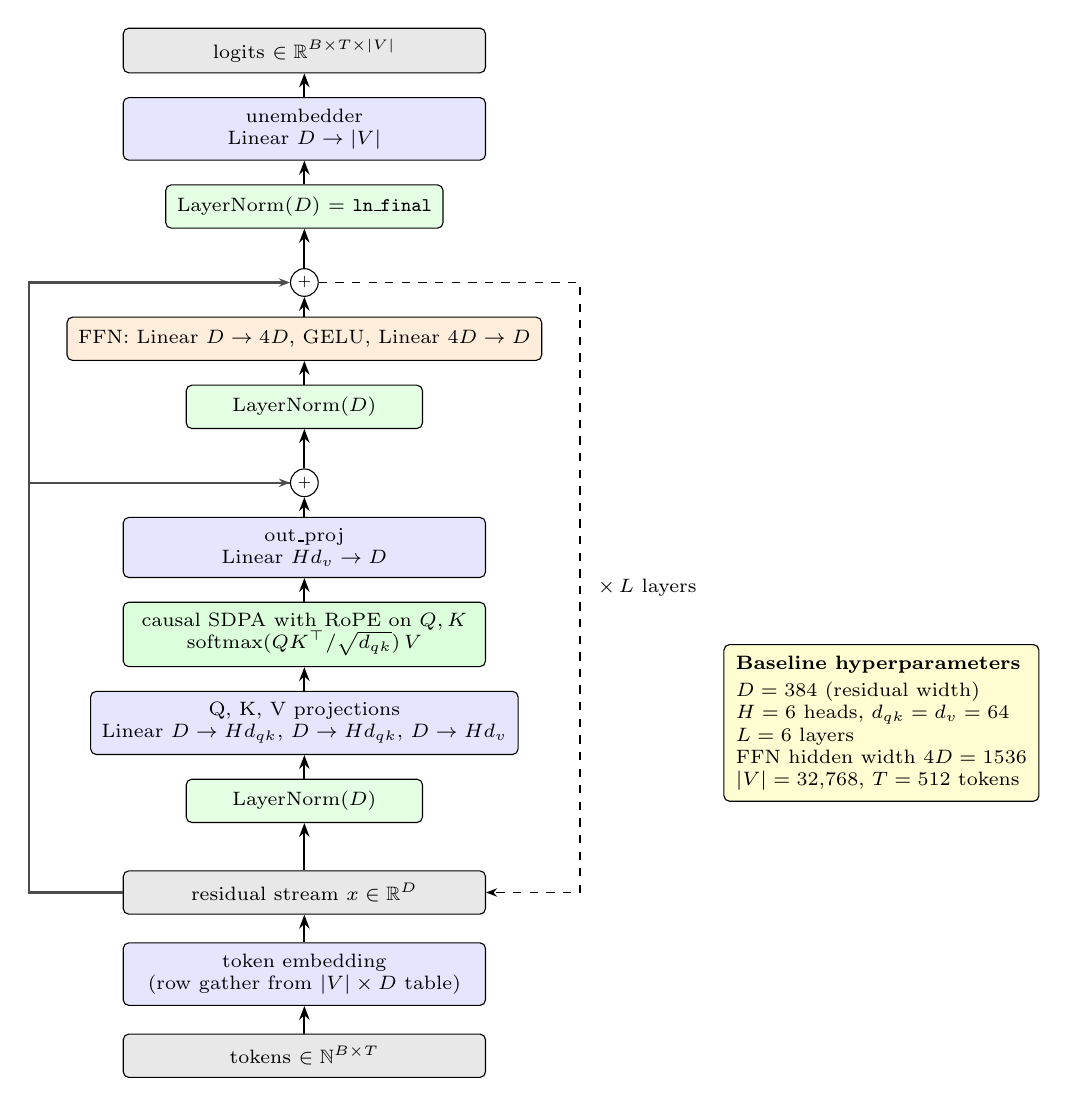
\begin{tikzpicture}[
    every node/.style={font=\scriptsize},
    box/.style={rectangle, draw, rounded corners=2pt, align=center, inner sep=4pt, fill=#1, minimum height=0.55cm, minimum width=4.6cm},
    box/.default=blue!8,
    proj/.style={box=blue!10},
    norm/.style={box=green!10, minimum width=3cm},
    op/.style={box=green!14, minimum width=4.6cm},
    ff/.style={box=orange!14, minimum width=4.6cm},
    stream/.style={box=gray!18, minimum width=4.6cm},
    arr/.style={-{Stealth[length=5pt]}, thick},
    add/.style={circle, draw, inner sep=1.2pt, fill=white, font=\tiny},
    sidearr/.style={-{Stealth[length=4pt]}, thick, gray!60!black},
    bracelabel/.style={font=\scriptsize, anchor=west},
]
% bottom-up vertical column
\node[stream] (tokens) at (0, 0) {tokens $\in \mathbb{N}^{B \times T}$};
\node[proj, above=0.35cm of tokens] (emb) {token embedding\\(row gather from $|V| \times D$ table)};
\node[stream, above=0.35cm of emb] (xres) {residual stream $x \in \mathbb{R}^D$};

% attention sub-block
\node[norm, above=0.6cm of xres] (ln1) {LayerNorm($D$)};
\node[proj, above=0.3cm of ln1] (qkv) {Q, K, V projections\\Linear $D \to H d_{qk}$, $D \to H d_{qk}$, $D \to H d_v$};
\node[op, above=0.3cm of qkv] (sdpa1) {causal SDPA with RoPE on $Q, K$\\$\mathrm{softmax}(QK^\top / \sqrt{d_{qk}})\, V$};
\node[proj, above=0.3cm of sdpa1] (oproj) {out\_proj\\Linear $H d_v \to D$};
\node[add, above=0.25cm of oproj] (a1) {$+$};

% FFN sub-block
\node[norm, above=0.5cm of a1] (ln2) {LayerNorm($D$)};
\node[ff, above=0.3cm of ln2] (ff) {FFN: Linear $D \to 4D$, GELU, Linear $4D \to D$};
\node[add, above=0.25cm of ff] (a2) {$+$};

% Final
\node[norm, above=0.5cm of a2] (lnf) {LayerNorm($D$) = \texttt{ln\_final}};
\node[proj, above=0.3cm of lnf] (head) {unembedder\\Linear $D \to |V|$};
\node[stream, above=0.3cm of head] (logits) {logits $\in \mathbb{R}^{B \times T \times |V|}$};

% column arrows
\draw[arr] (tokens) -- (emb);
\draw[arr] (emb) -- (xres);
\draw[arr] (xres) -- (ln1);
\draw[arr] (ln1) -- (qkv);
\draw[arr] (qkv) -- (sdpa1);
\draw[arr] (sdpa1) -- (oproj);
\draw[arr] (oproj) -- (a1);
\draw[arr] (a1) -- (ln2);
\draw[arr] (ln2) -- (ff);
\draw[arr] (ff) -- (a2);
\draw[arr] (a2) -- (lnf);
\draw[arr] (lnf) -- (head);
\draw[arr] (head) -- (logits);

% residuals (skip connections, side branches)
% Route both residual side branches through a common left rail at x = -3.5,
% well clear of the widest column boxes (4.6 cm wide -> west edge at -2.3).
\coordinate (leftrail) at (-3.5, 0);
\draw[sidearr] (xres.west) -- (xres.west -| leftrail) -- (a1.west -| leftrail) -- (a1.west);
\draw[sidearr] (a1.west)   -- (a1.west -| leftrail)   -- (a2.west -| leftrail) -- (a2.west);

% Dashed BLACK loop-return arrow: from a2 (the upper "+") back down to
% xres (the residual-stream entry of the layer), routed on the RIGHT at
% x=3.5 -- between the column boxes (right edge x=2.3) and the
% hyperparameter box (left edge x=4.9) -- so it does not collide with the
% left-side solid-gray residual side arrows. The "x L layers" label sits
% next to this arrow.
\coordinate (rrail) at (3.5, 0);
\draw[dashed, black, -{Stealth[length=4pt]}, line width=0.6pt]
    (a2.east) -- (a2.east -| rrail) -- (xres.east -| rrail) -- (xres.east);
\node[bracelabel, anchor=west, fill=white, inner sep=2pt] at ($(a2.east -| rrail)!0.5!(xres.east -| rrail) + (0.15,0)$) {$\times \, L$ layers};

% baseline hyperparams
\node[box=yellow!18, minimum width=4cm, right=2.6cm of qkv, align=left, anchor=west] (hp) {%
\textbf{Baseline hyperparameters}\\[2pt]
$D = 384$ (residual width)\\
$H = 6$ heads, $d_{qk} = d_v = 64$\\
$L = 6$ layers\\
FFN hidden width $4D = 1536$\\
$|V| = 32{,}768$, $T = 512$ tokens};

\end{tikzpicture}%
}%
\caption{Vanilla baseline transformer. One residual stream of width $D$. Each of $L$ layers contains a multi-head attention sub-block and a feed-forward network sub-block, each with its own LayerNorm and residual connection.}
\label{fig:vanilla}
\end{figure}

The baseline is a vanilla, RoPE-augmented transformer~\citep{vaswani2017attention,su2021roformer} with a separate unembedder (its own weight matrix, distinct from the token embedding), constructed by us as a deliberately simple comparison point on the nanochat data~\citep{karpathy_nanochat}. Nanochat itself proposes a more sophisticated GPT variant with several modern techniques; using that as the baseline would conflate the LUT-vs-non-LUT axis with the simple-vs-sophisticated-non-LUT axis. Vanilla-plus-RoPE is the simplest well-understood reference --- strong enough that matching it is a real signal, clean enough that the comparison isolates the LUT-vs-non-LUT axis from architectural improvements orthogonal to it.

\subsection{LUTGPT}
\label{ssec:lutgpt-arch}

\begin{figure}[!ht]
\centering
\scalebox{0.62}{%
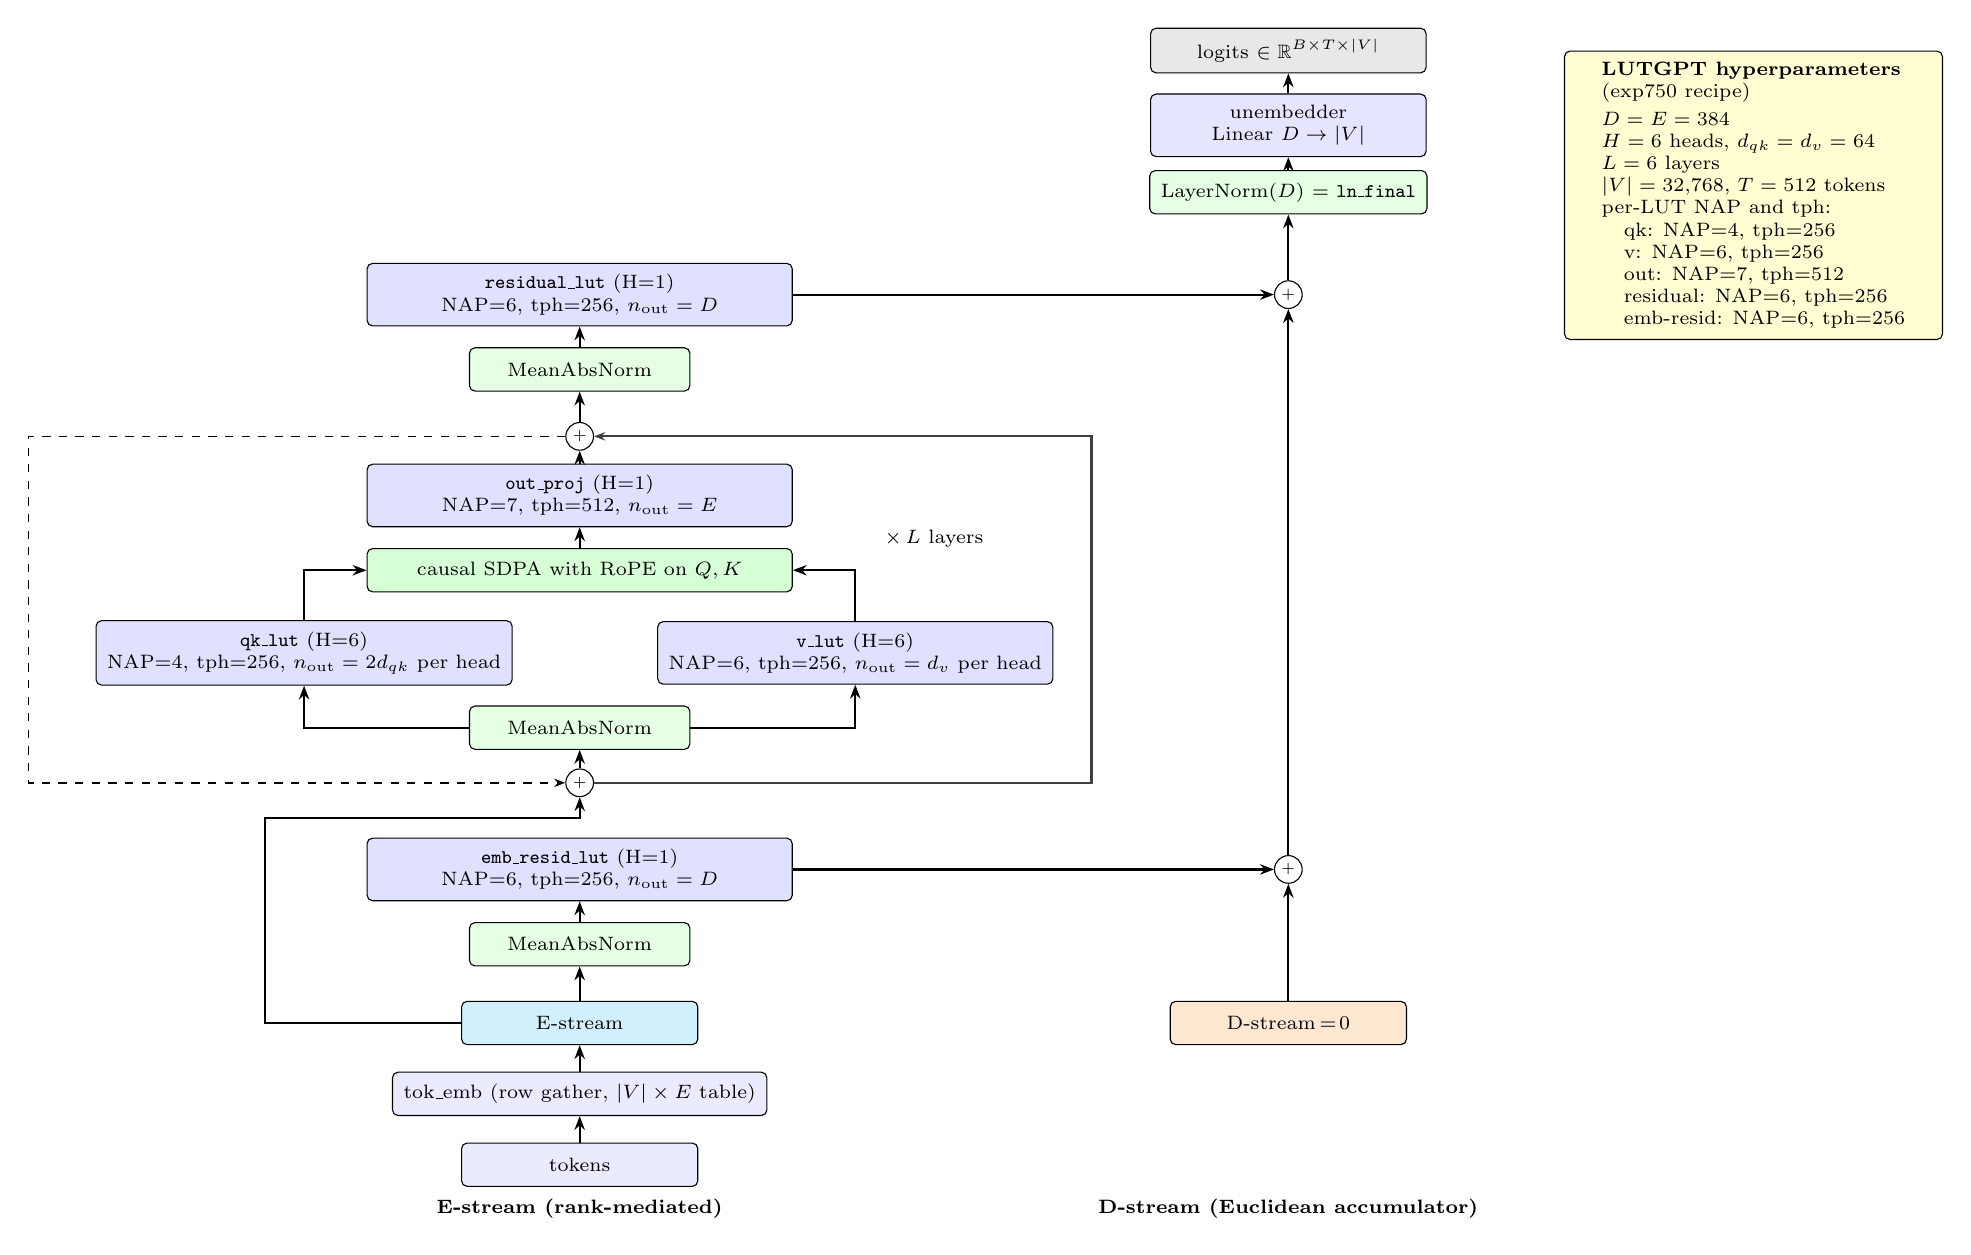
\begin{tikzpicture}[
    every node/.style={font=\scriptsize},
    box/.style={rectangle, draw, rounded corners=2pt, align=center, inner sep=4pt, fill=#1, minimum height=0.55cm},
    box/.default=blue!8,
    lut/.style={box=blue!12, minimum width=5.4cm},
    norm/.style={box=green!10, minimum width=2.8cm},
    op/.style={box=green!16, minimum width=5.4cm},
    emb/.style={box=blue!8, minimum width=3cm},
    estr/.style={box=cyan!18, minimum width=3cm},
    dstr/.style={box=orange!18, minimum width=3cm},
    final/.style={box=gray!14, minimum width=3cm},
    arr/.style={-{Stealth[length=5pt]}, thick},
    sidearr/.style={-{Stealth[length=4pt]}, thick, gray!50!black},
    add/.style={circle, draw, inner sep=1.2pt, fill=white, font=\tiny},
    streamlabel/.style={font=\scriptsize\bfseries, anchor=south},
]
% LUTGPT diagram, absolute coordinates.
% Main E-stream column at x=0. D-stream side rail at x=+5.5. Hyperparameter box at the right.

% Bottom: tokens + tok_emb + E-stream init
\node[emb]  (tokens)  at (0,  0.0) {tokens};
\node[emb]  (tokemb)  at (0,  0.9) {tok\_emb (row gather, $|V| \times E$ table)};
\node[estr] (xE0)     at (0,  1.8) {E-stream};
\node[dstr] (xD0)     at (9.0,1.8) {D-stream $\!=\!0$};

% emb_resid sub-block: MeanAbsNorm -> emb_resid_lut -> add to D
\node[norm] (mn0)     at (0,  2.8) {MeanAbsNorm};
\node[lut]  (embres)  at (0,  3.75){\texttt{emb\_resid\_lut} (H=1)\\NAP=6, tph=256, $n_{\text{out}}=D$};
\node[add]  (aD0)     at (9.0,3.75){$+$};

\draw[arr] (tokens) -- (tokemb);
\draw[arr] (tokemb) -- (xE0);
\draw[arr] (xE0)    -- (mn0);
\draw[arr] (mn0)    -- (embres);
\draw[arr] (embres.east) -- (aD0.west);
\draw[arr] (xD0)    -- (aD0);

% E-stream block entry "+" marker (inside the loop, just above its south edge).
% Represents the E-stream value that ENTERS the layer -- either xE0 from the
% tok_emb output (first iteration) or the previous layer's aE (subsequent
% iterations, via the dashed loop-return on the left).
\node[add] (aEin) at (0,   4.85) {$+$};

% Attention sub-block on E-stream (qk_lut and v_lut are parallel, on the same
% row). Each LUT is 4.0cm wide and centred at +-3.5 so there is a clear 3.0cm
% gap between them at x in [-1.5, +1.5] -- well above the MeanAbsNorm box
% (width 2.8cm) so the side-entry arrows can route through this gap.
\node[norm] (mn1)     at (0,  5.55) {MeanAbsNorm};
\node[lut, minimum width=4.0cm] (qklut) at (-3.5, 6.5) {\texttt{qk\_lut} (H=6)\\NAP=4, tph=256, $n_{\text{out}}=2 d_{qk}$ per head};
\node[lut, minimum width=4.0cm] (vlut)  at ( 3.5, 6.5) {\texttt{v\_lut} (H=6)\\NAP=6, tph=256, $n_{\text{out}}=d_v$ per head};
\node[op]   (sdpa)    at (0,  7.55) {causal SDPA with RoPE on $Q, K$};
\node[lut]  (op2)     at (0,  8.5)  {\texttt{out\_proj} (H=1)\\NAP=7, tph=512, $n_{\text{out}}=E$};
\node[add]  (aE)      at (0,  9.25) {$+$};

% E-stream main flow: xE0 (the tok_emb output) goes UP into the first layer's
% entry "+" (aEin). emb_resid_lut is a SIDE branch that reads xE0 and writes
% to the D-stream; it does NOT feed the E-stream. The arrow is routed LEFT
% around the emb_resid sub-block (mn0 + embres at x=0) at x=-4.0, then back
% RIGHT, and enters aEin from the SOUTH so it does not overlap with the
% dashed loop-return arrow that enters aEin from the WEST. The horizontal
% segment sits at y=4.25 (just above embres top at ~4.15) so the final
% vertical approach into aEin.south is clearly visible.
\draw[arr] (xE0.west) -- (-4.0, 1.8) -- (-4.0, 4.4) -- (0, 4.4) -- (aEin.south);
\draw[arr] (aEin)   -- (mn1);
% Orthogonal split: arrows leave mn1 from its SIDES (east / west), turn 90 deg,
% and arrive at the SOUTH of qk_lut and v_lut.
\draw[arr] (mn1.west) -| (qklut.south);
\draw[arr] (mn1.east) -| (vlut.south);
% Orthogonal join: arrows leave qk_lut / v_lut from their TOP, go vertical up,
% then turn 90 deg and arrive at the SIDES of sdpa (west and east).
\draw[arr] (qklut.north) |- (sdpa.west);
\draw[arr] (vlut.north)  |- (sdpa.east);
\draw[arr] (sdpa)   -- (op2);
\draw[arr] (op2)    -- (aE);
% E-stream residual: from the entry "+" (aEin), around the attention sub-block
% on the RIGHT at x=6.5 -- between v_lut.east (5.5) and the D-stream column
% (centred at 9.0, west edge 7.5) -- into the upper "+" (aE).
\coordinate (e_resrail) at (6.5, 0);
\draw[sidearr] (aEin.east) -- (aEin.east -| e_resrail) -- (aE.east -| e_resrail) -- (aE.east);

% residual_lut sub-block: MeanAbsNorm -> residual_lut -> add to D
\node[norm] (mn2)     at (0, 10.1)  {MeanAbsNorm};
\node[lut]  (reslut)  at (0, 11.05) {\texttt{residual\_lut} (H=1)\\NAP=6, tph=256, $n_{\text{out}}=D$};
\node[add]  (aD1)     at (9.0,11.05){$+$};

\draw[arr] (aE)     -- (mn2);
\draw[arr] (mn2)    -- (reslut);
\draw[arr] (reslut.east) -- (aD1.west);
% D-stream flow: from aD0 (init, outside loop) straight into the upper "+"
% (aD1). The D-stream just accumulates per-layer residual_lut contributions;
% there is no second input being summed before aD1, so no separate entry "+".
\draw[arr] (aD0) -- (aD1);

% Dashed BLACK loop-return arrows: one per stream, connecting the upper "+"
% of each stream back down to its entry "+". The "x L layers" label sits on
% the E-stream loop arrow's vertical segment.
% E-stream loop-return: routed on the left at x=-7.0, well clear of qk_lut
% (its west edge is at -5.5).
\coordinate (e_looprail) at (-7.0, 0);
\draw[dashed, black, -{Stealth[length=4pt]}, line width=0.6pt]
    (aE.west) -- (aE.west -| e_looprail) -- (aEin.west -| e_looprail) -- (aEin.west);
% "x L layers" label is placed horizontally between the E-stream column
% (x=0, with sdpa/op2 extending to x=+-2.7) and the D-stream column (x=9.0,
% with the classifier boxes whose west edge sits at 7.25). x=4.5 is the
% midpoint of the gap; y matches the vertical midpoint of both loop arrows
% so the single label visually applies to both.
\node[font=\scriptsize, anchor=center, fill=white, inner sep=2pt]
    at (4.5, 7.95)
    {$\times \, L$ layers};
% D-stream has no loop-return arrow: per-layer residual_lut output is added at
% aD1 and that value flows straight into the next layer's aD1; no separate
% join point is needed.

% Final classifier path on D-stream. Styled to match the vanilla figure's
% LayerNorm (green!10), unembedder (blue!10), logits (gray!18 stream).
\node[box=green!10, minimum width=3.5cm, minimum height=0.55cm,
      rounded corners=2pt, draw, align=center, inner sep=4pt]
      (lnf) at (9.0,12.35) {LayerNorm($D$) = \texttt{ln\_final}};
\node[box=blue!10, minimum width=3.5cm, minimum height=0.55cm,
      rounded corners=2pt, draw, align=center, inner sep=4pt]
      (head) at (9.0,13.2) {unembedder\\Linear $D \to |V|$};
\node[box=gray!18, minimum width=3.5cm, minimum height=0.55cm,
      rounded corners=2pt, draw, align=center, inner sep=4pt]
      (logits) at (9.0,14.15) {logits $\in \mathbb{R}^{B \times T \times |V|}$};

\draw[arr] (aD1) -- (lnf);
\draw[arr] (lnf) -- (head);
\draw[arr] (head)-- (logits);

% Stream labels
\node[streamlabel] at (0,  -0.8) {E-stream (rank-mediated)};
\node[streamlabel] at (9.0,-0.8) {D-stream (Euclidean accumulator)};

% Hyperparameter box
\node[box=yellow!18, align=left, minimum width=4.8cm, anchor=north west] at (12.5, 14.15) (hp) {%
\textbf{LUTGPT hyperparameters}\\(exp750 recipe)\\[2pt]
$D = E = 384$\\
$H = 6$ heads, $d_{qk} = d_v = 64$\\
$L = 6$ layers\\
$|V| = 32{,}768$, $T = 512$ tokens\\
per-LUT NAP and tph:\\
\quad qk: NAP=4, tph=256\\
\quad v: NAP=6, tph=256\\
\quad out: NAP=7, tph=512\\
\quad residual: NAP=6, tph=256\\
\quad emb-resid: NAP=6, tph=256};

\end{tikzpicture}%
}%
\caption{LUTGPT (exp750 recipe). Two residual streams: the E-stream (centre, width $E$) is the rank-mediated backbone, mutated only by the per-layer \texttt{out\_proj}; the D-stream (right, width $D$) is the Euclidean accumulator, written by \texttt{emb\_resid\_lut} once and by \texttt{residual\_lut} once per layer, read by the linear unembedder. There is no FFN. The two streams are at the same width ($E = D = 384$); the split is structural, not size-based --- see Section~\ref{ssec:dual-stream}.}
\label{fig:lutgpt}
\end{figure}

\subsection{Methodological commitment: baseline matching}
\label{ssec:matching}

The two architectures share every hyperparameter that sits at a fair-comparison interface:

\begin{itemize}[leftmargin=*,topsep=2pt,itemsep=1pt]
\item $D = 384$ --- the residual stream width on the side feeding the linear unembedder. Matched so our unembedder operates at the same width as vanilla's.
\item $\dqk = 64$ per head --- Q/K dimension at SDPA. Matched so the attention machinery sees the same shape of $Q, K$.
\item Vocab size 32{,}768 and sequence length 512 --- inherited from nanochat. $H = 6$ heads and $L = 6$ layers --- our choices, picked at the typical small-GPT scale for fast iteration, and matched on both sides.
\item Separate embedding and unembedding matrices on both sides; ClimbMix data shards, BPE tokeniser, RoPE positional encoding, AdamW for non-LUT parameters --- inherited unchanged.
\end{itemize}

The LUTGPT-specific dimensions ($E = 384$, $\dv = 64$, the per-LUT NAP and $\mathrm{tph}$) are then chosen freely, and motivated in Section~\ref{ssec:lutgpt-hyperparams} below.

\subsection{Dual residual stream}
\label{ssec:dual-stream}

The intuition for the dual stream is: keep the vanilla residual stream as-is, and put a different backbone next to it. A vanilla transformer maintains one residual stream of width $D$; the backbone is the $L$-layer stack of attention + FFN blocks, and after each layer the backbone adds an update to the residual stream. The classifier reads the residual stream at the top. LUTGPT keeps exactly this picture, but swaps the backbone.

\begin{itemize}[leftmargin=*,topsep=2pt,itemsep=1pt]
\item \textbf{D-stream} (width $D = 384$): the standard residual stream. Same role as vanilla's residual stream and the same width. It is initialised at the embedding interface by \texttt{emb\_resid\_lut}, gets a contribution from each layer (added by \texttt{residual\_lut}), and is read at the top by \texttt{ln\_final} and the linear unembedder, which produce the logits. From the classifier's point of view, LUTGPT looks like a vanilla transformer.

\item \textbf{E-stream} (width $E = 384$): the rank-coded backbone that produces the per-layer contributions. Where vanilla's backbone is dense matmuls (Q/K/V projections, attention, FFN), LUTGPT's backbone is a rank-mediated computation graph of LUTs. The E-stream is the value the backbone passes between its own layers; every consumer of the E-stream is a LUT preceded by \texttt{MeanAbsNorm}, so the information that propagates along E is rank-coded (only the order of coordinates matters to the next LUT). At each layer, the backbone exports a contribution into the D-stream via \texttt{residual\_lut}.
\end{itemize}

The split is not for capacity. The two streams have the same dimension. The split exists because the backbone (which wants to operate on ranks) and the classifier (which wants Euclidean magnitudes) want different kinds of representation, and a single residual stream would have to satisfy both simultaneously. Keeping them separate lets each be exactly what it needs to be.

\subsection{Three roles for LUTs at the interfaces}

Every LUT in LUTGPT reads from the E-stream and emits a row from its weight table, but what \emph{happens} to that row downstream depends on the LUT's role. Four distinct interface patterns appear:

\begin{itemize}[leftmargin=*,topsep=2pt,itemsep=1pt]
\item \textbf{\texttt{qk\_lut} $\to$ SDPA dot product.} The dot product $Q \cdot K^\top$ is the one operation in the model that strictly requires real-valued magnitudes; there is no rank-only way to compute a similarity that respects scale. The Q and K LUTs are accordingly the \emph{adapters} from the rank-mediated E-stream into a real-valued representation that SDPA can read. RoPE is applied on top.

\item \textbf{\texttt{v\_lut} $\to$ attention convex sum $\to$ \texttt{out\_proj}.} The V LUT is structurally different. Its output is multiplied by the soft attention weights, which are non-negative and sum to 1, giving a convex combination of V rows that then flows into the next LUT in line. This convex mixing is the \emph{only} operation in the model that takes LUT outputs and recombines them \emph{before} a downstream LUT re-decodes them; the V LUT must be trained so its outputs remain mixable, i.e., convex combinations of plausible V rows stay inside a rank-decodable region for \texttt{out\_proj}. The V LUT is rank-coded in input, rank-coded (via mixability) in output.

\item \textbf{\texttt{out\_proj} $\to$ E-stream $\to$ next layer's LUTs.} \texttt{out\_proj} is an ordinary LUT in this scheme --- not a reverse adapter. Its input is the SDPA output, which by the V-LUT mixability argument above is a convex combination of rank-decodable rows and therefore still lies in the rank-decodable region. \texttt{out\_proj} reads it with sign-pack like any other LUT, and its row gather is added to the E-stream as the layer's attention contribution.

\item \textbf{\texttt{emb\_resid\_lut}, \texttt{residual\_lut} $\to$ D-stream $\to$ linear unembedder.} \texttt{emb\_resid\_lut} (once, at the embedding interface) and \texttt{residual\_lut} (once per layer) write into the D-stream, which is read by the linear unembedder. Both are adapters from a rank-coded E-stream input to a real-valued contribution to the D-stream, in the same family as Q/K.
\end{itemize}

\subsection{No separate FFN}
\label{ssec:no-ffn}

The vanilla layer in Figure~\ref{fig:vanilla} carries two computational blocks: an attention sub-block (Q/K/V projections, attention, output projection) and an FFN afterward, with the FFN typically holding the bulk of the per-layer parameters. LUTGPT (Figure~\ref{fig:lutgpt}) has no separate FFN. The \texttt{out\_proj} LUT absorbs that role.

In vanilla, \texttt{out\_proj} is a thin linear projection from concatenated attention heads to the residual width, and the FFN that follows is where most of the per-layer expressivity lives. In LUTGPT, \texttt{out\_proj} is itself a multi-head LUT: it reads the post-attention representation, decodes it through anchor-pair sign comparisons, and gathers from a large learnt weight table to produce the residual update. The expressivity that the vanilla FFN provides through wide hidden linear layers and a nonlinearity is provided here by the LUT lookup mechanism itself --- a learned discrete-indexed function with $K \cdot \dout$ degrees of freedom per table, capturing nonlinearity through the row gather. Per-layer evidence accumulation into the classifier path is then a separate role, taken by \texttt{residual\_lut} writing into the D-stream (a role that does not exist in the vanilla architecture, since vanilla shares a single residual stream for both the backbone and the classifier input).

\subsection{LUT-specific hyperparameter choices}
\label{ssec:lutgpt-hyperparams}

The dimensions matched against vanilla ($D$, $\dqk$, $H$, vocab, context length) are fixed by the baseline-matching commitment of Section~\ref{ssec:matching}. The remaining choices are LUT-specific:

\paragraph{Backbone width $E$ and per-head dimensions $\dqk$, $\dv$.} The constraint $E = H \cdot \dv$ is always enforced so the SDPA output (concatenation of $H$ heads of $\dv$ values) lands at the E-stream width with no reshape and \texttt{out\_proj} reads an $E$-dimensional input. We report two configurations (Section~\ref{sec:experiments}):
\begin{itemize}[leftmargin=*,topsep=2pt,itemsep=1pt]
\item \textbf{Full-width backbone} (\texttt{exp754}): $\dv = \dqk = 64$ and $E = D = 384$. Per-head $Q$, $K$, and $V$ dimensions all match the vanilla baseline; the backbone runs at the same width as the D-stream and the unembedder readout.
\item \textbf{Narrow backbone} (\texttt{exp755}): $\dv = 32$ and $E = 192$, with $\dqk = 64$ held to the baseline. The LUT-bearing backbone is half-width while the D-stream stays at $D = 384$ for the unembedder readout.
\end{itemize}

These two configurations together test the asymmetric-architecture claim of Section~\ref{ssec:dual-stream}: the rank-coded stream where the LUTs compute is allowed to be narrow, while the Euclidean accumulator stays wide for the unembedder. The remaining LUT-specific choices (anchor pairs per table, $\mathrm{tph}$, qk-lut sharing) are identical across both configurations.

\paragraph{Anchor pairs per table (NAP).} Larger NAP gives the LUT more discrimination capacity (each table has $K = 2^{\mathrm{NAP}}$ rows), at quadratic cost in the soft surrogate backward (a full $K$-way softmax per (sample, table)). We use NAP $\in \{4, 6, 7\}$ in LUTGPT, scaled to the role of each LUT:

\begin{itemize}[leftmargin=*,topsep=2pt,itemsep=1pt]
\item $\mathrm{NAP} = 4$ ($K = 16$) for \texttt{qk\_lut}. The qk\_lut feeds the SDPA dot product. Its job is to make Q and K discriminative enough that softmax-attention picks the right positions; the dot-product score and the downstream attention weights then carry the fine-grained signal.

The smaller NAP here is also a plasticity choice. Attention patterns emerge during training and keep changing throughout the run, so the Q/K projections must stay flexible end-to-end. In a vanilla transformer Q and K come from dense linear projections, and every backward step updates every weight; gradients are uniformly strong. In LUTGPT each token-level lookup touches only one row of a $K \times \dout$ table (two in hybrid-smooth), so the per-row gradient sees only a fraction $\sim B / K$ of the batch per step. Larger $K$ makes the per-row update count smaller and trainability deteriorates --- at the SDPA interface, where the layer has to relearn its own attention pattern continuously, this is the most painful place for that to happen. Smaller $K$ keeps every Q/K row in the active-training regime; $K = 16$ is the smallest value at which the family still has enough distinct Q/K vectors to express useful attention patterns in our experiments.
\item $\mathrm{NAP} = 6$ ($K = 64$) for \texttt{v\_lut}, \texttt{residual\_lut}, and \texttt{emb\_resid\_lut}. Wider tables at the streams where the LUT output directly populates a per-token vector that downstream layers (or the unembedder) read at full width.
\item $\mathrm{NAP} = 7$ ($K = 128$) for \texttt{out\_proj}. Out-proj absorbs the FFN's role (Section~\ref{ssec:no-ffn}) and is the single LUT in the layer that has to carry the bulk of the per-layer transformation; we give it the largest row count.
\end{itemize}

\paragraph{Tables per head $\mathrm{tph}$.} Each LUT's per-head output is the sum of its $\mathrm{tph}$ table outputs (Section~\ref{ssec:setup}). Larger $\mathrm{tph}$ gives the layer more capacity at linear cost in the forward and the soft backward. We use $\mathrm{tph} = 256$ for the qk, v, residual, and emb-resid LUTs (a common default), and $\mathrm{tph} = 512$ for \texttt{out\_proj} specifically, because \texttt{out\_proj} absorbs the FFN's role and is the single LUT in the layer carrying the bulk of the per-layer expressivity.

\paragraph{qk\_lut sharing for Q and K.} A single LUT generates both Q and K projections by emitting an output of width $2 \dqk$ per head, then splitting the output into $Q$ and $K$ inside the layer. This is a small economy: Q and K are needed at the same time, at the same per-head width, and from the same input, so they share the lookup overhead.

\FloatBarrier

% =========================================================================
\section{Training recipe}
\label{sec:training}

LUT weight tables are trained with Lion~\citep{chen2023lion}; all non-LUT parameters --- the token embedding, the unembedder, the layer norms, the per-LUT temperatures --- are trained with AdamW~\citep{loshchilov2017decoupled}. The choice is a memory choice, not a quality choice. Lion stores one momentum buffer per parameter; AdamW stores two ($m$ and $v$). For a model that has roughly $5$--$8\times$ as many parameters as the matched vanilla baseline (depending on backbone width), the optimiser state on LUT weights is a meaningful fraction of training memory. Empirically, Lion matches AdamW on LUT-weight quality --- comparable validation loss, never worse on our recipes --- at half the per-parameter state. We use Lion for the LUT tables because of this memory saving, and AdamW for non-LUT parameters because that is the conventional default and we do not benefit from changing it.

The default schedule is a single cosine decay over the full 16{,}000-step run with a 10\% linear warmup, peaking at $\mathrm{lr}_{\mathrm{adam}} = 3 \cdot 10^{-4}$ for AdamW (non-LUT parameters) and $\mathrm{lr}_{\mathrm{lion}} = 2 \cdot 10^{-4}$ for Lion (LUT weights), both decaying to $0.1\times$ peak. Effective batch is held constant across the run at $48 \cdot 512 = 24{,}576$ tokens per step. Gradient clipping is \texttt{clip\_grad\_norm} to $1.0$ over all trainable parameters.

The forward mode is held fixed within a single run. Whether to train in hybrid-smooth (smaller training loss, larger soft-to-hard eval gap) or in hard (larger training loss, deployable as-is on a magnitude-blind hard forward) is a model choice; we report both in Section~\ref{sec:experiments}.

% =========================================================================
\section{Efficiency analysis and the hardware bet}
\label{sec:efficiency}

\subsection{GPU wall-clock cost}

LUTGPT is slower than the matched vanilla baseline on training and on inference, on every GPU we measured. Reasons:

\begin{itemize}[leftmargin=*,topsep=2pt,itemsep=1pt]
\item The model has $5$--$8\times$ more parameters than the matched vanilla baseline ($7.7\times$ at the full-width backbone, $4.9\times$ at the narrow backbone); even at proportionally lower fetch-bandwidth-per-token, the absolute compute is greater.
\item The LUT backward path executes a soft-surrogate matmul (sparse selection mass times grad output) for every layer in every step; this is dense in compute even though sparse in selection.
\item LUT forward gathers do not use tensor cores; on consumer and datacenter GPUs the model is HBM-bandwidth-bound on the LUT layers while the SDPA layers happily use bf16 tensor cores. The mix is not what current GPUs are tuned for.
\end{itemize}

We report wall-clock numbers as found and do not promise improvements achievable on this hardware class.

\subsection{Bandwidth and active-parameter profile}

The properties that justify presenting the family despite the GPU result are two:

\begin{itemize}[leftmargin=*,topsep=2pt,itemsep=1pt]
\item \textbf{HBM read per token, trunk.} A LUTGPT layer reads $H \cdot \mathrm{tph} \cdot D_{\mathrm{out}} \cdot \mathrm{bytes}$ for the gathers --- one row per table per token. Summed across all LUTs in the trunk and across $L = 6$ layers, the full-width backbone (\texttt{exp754}) reads $\sim 7.3$\,MB per token, against $\sim 21.2$\,MB for the vanilla matmul backbone at $D = 384$ --- a factor of $\sim 2.9$. The narrow backbone (\texttt{exp755}) reads $\sim 5.5$\,MB per token --- a factor of $\sim 3.8$. The factor scales further at larger $K = 2^N$: bandwidth is independent of $K$, while vanilla's projection cost scales with output width.
\item \textbf{Active parameters per token.} A vanilla projection activates every weight per token. A LUTGPT projection activates exactly $H \cdot \mathrm{tph}$ rows per token --- a small, predictable subset of $K \cdot H \cdot \mathrm{tph}$ total. The active-parameter fraction is below 5\% per token in both configurations, and the active set is decided by sign comparisons, not by data-dependent computation.
\end{itemize}

\paragraph{Compression density.} To make the bandwidth picture explicit, define
\[
\mathrm{compression\ density} \;=\; \frac{\text{stored parameters}}{\text{HBM bytes fetched per token}}.
\]
This measures how much model capacity a layer holds per unit of memory traffic, and is the relevant metric on bandwidth-bound hardware. For a dense linear layer every weight is fetched exactly once per token, so the compression density is fixed at $1/b$ params per byte (where $b$ is the number of bytes per stored value, e.g.\ $b = 2$ at bf16) --- a ceiling that no choice of width can raise. For a multi-head LUT each table holds $K$ rows but only one row per (table, token) is fetched at inference, so the compression density is $K/b$ params per byte: the table holds $K \times$ more weights than a dense layer would at the same per-token bandwidth budget. Doubling $K$ doubles the stored parameters of a LUT but does not change its per-token bytes fetched. Aggregated across the LUTGPT trunk against vanilla's matmul backbone, the compression density is roughly $20\times$ higher in both configurations of Section~\ref{sec:experiments}.

On hardware that fetches only the active rows from a compressed indexed store --- the class of accelerator we have in mind --- the parameter count stops being a cost. The dense linear unembedder (a $D \times |V|$ matmul, identical to vanilla and accounting for the majority of total per-token HBM read in either model) is the dominant remaining matmul interface; we leave it as one of the open problems in Section~\ref{sec:open}.

\subsection{The bet}

The bet is straightforward: \emph{the LUT family is presented as an architecture that maps cleanly onto rank-coded sparse-lookup hardware, and we conjecture that hardware of this kind would make the family competitive or preferred at scale.} We are not claiming such hardware exists. We are presenting the architectural properties that would make it matter if it did --- a low HBM read per token and a sparse, predictable active-parameter set --- and arguing that they justify holding the LUT family open as a research direction even when current GPUs make it look uneconomical.

% =========================================================================
\section{Experiments}
\label{sec:experiments}

\subsection{Data, budget, and hardware}
\label{ssec:exp-setup}

All runs in this section use the optimiser and learning-rate recipe of Section~\ref{sec:training} (AdamW for non-LUT parameters; Lion for LUT weights; warmup-cosine schedule; \texttt{clip\_grad\_norm} to $1.0$). The remaining setup that is common to every experiment:

\begin{itemize}[leftmargin=*,topsep=2pt,itemsep=1pt]
\item \textbf{Data and tokeniser.} The \texttt{nanochat} pre-training text mix (a ClimbMix derivative) tokenised with the RustBPE tokeniser, $|V| = 32{,}768$. Context length $T = 512$.
\item \textbf{Compute budget.} $n_{\mathrm{steps}} = 16{,}000$ at total batch $48 \cdot 512 = 24{,}576$ tokens per step, i.e.\ $\sim 3.93 \cdot 10^8$ training tokens per run. The vanilla baseline uses device batch $48$ with $\mathrm{grad\_accum} = 1$; LUTGPT uses device batch $24$ with $\mathrm{grad\_accum} = 2$ for memory reasons. The effective batch is identical in both cases.
\item \textbf{Hardware.} Single H100 GPU per run. The vanilla baseline completes in $\sim 37$ minutes; the full-width LUTGPT run (\texttt{exp754}) completes in $\sim 6.3$ hours; the narrow-backbone LUTGPT run (\texttt{exp755}) completes in $\sim 5.4$ hours.
\item \textbf{Evaluation metric.} Validation loss is reported in \emph{bits per byte} (bpb): the per-token cross-entropy on the held-out validation text, summed in bits over the validation tokens and divided by the total raw-byte count of the same text,
\[
\mathrm{bpb} \;=\; \frac{-\sum_i \log_2 p(t_i \mid t_{<i})}{\sum_i \mathrm{bytes}(t_i)},
\]
where $\mathrm{bytes}(t_i)$ is the number of UTF-8 bytes the BPE token $t_i$ represents. Dividing by raw bytes rather than tokens makes the metric tokeniser-independent: a model with a $32{,}768$-vocab BPE and one with a different vocabulary on the same text are directly comparable. Lower is better. We use the \texttt{evaluate\_bpb} routine from \texttt{nanochat}, averaged over \texttt{eval\_steps}\,$=10$ micro-batches at the same context length as training.
\end{itemize}

\subsection{Vanilla baseline (\texttt{exp709})}
\label{ssec:exp-baseline}

The vanilla reference is the untied \texttt{MinimalGPT+RoPE} architecture of Section~\ref{ssec:baseline}: pre-norm transformer block (\texttt{LayerNorm} $\to$ SDPA attention $\to$ residual; \texttt{LayerNorm} $\to$ GELU MLP $\to$ residual), residual width $D = 384$, depth $L = 6$, $H = 6$ heads with per-head dimension $64$, FFN hidden $= 4D$, untied unembedder. All Linear and Embedding weights are initialised from $\mathcal{N}(0, 0.02^2)$; the attention output projection and the second MLP linear are zero-initialised, so every residual branch starts at zero and the model begins as the identity map on the embedding.

At $35.79$\,M parameters this is the standard nanoGPT-class point of comparison and our headline number to beat (or land near). The final validation loss after $16{,}000$ steps is

\begin{center}
\texttt{exp709}: $\quad$ \textbf{val\_bpb $= 1.1922$} $\quad$ at $35.79$\,M parameters.
\end{center}

\subsection{LUTGPT, full-width backbone (\texttt{exp754})}
\label{ssec:exp-headline}

The headline LUTGPT configuration uses the architecture of Section~\ref{ssec:lutgpt-arch} at full backbone width.

\begin{itemize}[leftmargin=*,topsep=2pt,itemsep=1pt]
\item $E = D = 384$, $L = 6$, $H = 6$, $\dqk = \dv = 64$.
\item Anchor-pairs per table (Section~\ref{ssec:lutgpt-hyperparams}): \texttt{qk\_lut} $N{=}4$ at $\mathrm{tph}{=}256$; \texttt{v\_lut} $N{=}6$ at $\mathrm{tph}{=}256$; \texttt{out\_proj} $N{=}7$ at $\mathrm{tph}{=}512$; \texttt{residual\_lut} and \texttt{emb\_resid\_lut} $N{=}6$ at $\mathrm{tph}{=}256$.
\item Forward mode \texttt{hybrid\_smooth} with backward mode \texttt{dense\_K}, held fixed for all $16{,}000$ steps.
\end{itemize}

\begin{center}
\texttt{exp754}: $\quad$ \textbf{val\_bpb $= 1.1842$} $\quad$ at $276.8$\,M parameters.
\end{center}

This is $8.0$\,mb below the vanilla baseline at $7.7\times$ the parameter count. We are not claiming a parameter-efficient win; the LUT family carries more parameters by construction (a $K \cdot \mathrm{tph}$ table per output channel against a single dense weight matrix). What this result establishes is that at matched data and matched training-token budget, the LUT family lands on the same side of the vanilla curve --- a result we did not have access to before this run.

\subsection{LUTGPT, narrow backbone (\texttt{exp755})}
\label{ssec:exp-narrow}

A second LUTGPT configuration narrows the backbone --- the rank-coded stream where the LUTs actually compute --- to half-width, keeping the Euclidean D-stream wide for the unembedder readout.

\begin{itemize}[leftmargin=*,topsep=2pt,itemsep=1pt]
\item $E = 192$ (backbone), $D = 384$ (D-stream accumulator), $L = 6$, $H = 6$, $\dqk = 64$, $\dv = 32$.
\item All other settings identical to \texttt{exp754} (anchor-pair budget, forward/backward modes, training recipe).
\end{itemize}

\begin{center}
\texttt{exp755}: $\quad$ \textbf{val\_bpb $= 1.2044$} $\quad$ at $176.2$\,M parameters.
\end{center}

This is $12.2$\,mb above the vanilla baseline at $4.9\times$ the parameter count. The point of this run is structural rather than headline: the LUT-bearing backbone can be halved in width with only a $\sim 20$\,mb loss penalty relative to the full-width \texttt{exp754}, while the wide D-stream accumulator (read only by the linear unembedder) is preserved unchanged. This validates the asymmetric architecture of Section~\ref{ssec:dual-stream}: most of the LUT compute belongs in a narrow rank-coded stream, and only the unembedder needs a wide Euclidean input.

\subsection{The soft-to-hard gap}
\label{ssec:exp-soft-hard}

Both \texttt{exp754} and \texttt{exp755} are trained with the hybrid-smooth forward (Section~\ref{ssec:forward}). Hybrid-smooth eval is the in-distribution measurement of a hybrid-smooth-trained model; hard eval is the measurement under the magnitude-blind forward that maps directly to rank-coded sparse-lookup hardware. The gap between them is the structural cost of hardware-targetedness.

We measure two things: (i) the soft-to-hard gap on the same trained checkpoint, and (ii) the alternative of training in hard mode from scratch.

\begin{center}
\begin{tabular}{lcccr}
\toprule
\textbf{run} & \textbf{params} & \textbf{trained mode} & \textbf{eval mode} & \textbf{val\_bpb} \\
\midrule
\texttt{exp754} & $276.8$\,M & \texttt{hybrid\_smooth} & \texttt{hybrid\_smooth} & $1.1842$ \\
\texttt{exp754} & $276.8$\,M & \texttt{hybrid\_smooth} & \texttt{hard}           & $1.2498$ \\
\texttt{exp752} & $276.8$\,M & \texttt{hard}           & \texttt{hard}           & $1.2162$ \\
\midrule
\texttt{exp755} & $176.2$\,M & \texttt{hybrid\_smooth} & \texttt{hybrid\_smooth} & $1.2044$ \\
\texttt{exp755} & $176.2$\,M & \texttt{hybrid\_smooth} & \texttt{hard}           & $1.2778$ \\
\texttt{exp756} & $176.2$\,M & \texttt{hard}           & \texttt{hard}           & $1.2301$ \\
\bottomrule
\end{tabular}
\end{center}

Two observations.

\paragraph{The soft-trained model loses 65--73\,mb when forced into hard forward at eval time.} \texttt{exp754} drops from $1.1842$ to $1.2498$ ($+65.6$\,mb) when its forward is switched to hard at eval; \texttt{exp755} drops from $1.2044$ to $1.2778$ ($+73.4$\,mb). The hybrid-smooth-trained model has learnt to lean on the small-magnitude top-$k$ blending that the hard forward discards. The soft-to-hard pipeline at eval time is not free.

\paragraph{Training in hard mode from scratch closes most of that gap.} \texttt{exp752} (same architecture as \texttt{exp754}, trained \emph{in} hard mode) lands at $1.2162$ --- $33.6$\,mb below \texttt{exp754}'s hard-eval number. \texttt{exp756} (same architecture as \texttt{exp755}, hard-trained) lands at $1.2301$ --- $47.7$\,mb below \texttt{exp755}'s hard-eval number.

\begin{figure}[!ht]
\centering
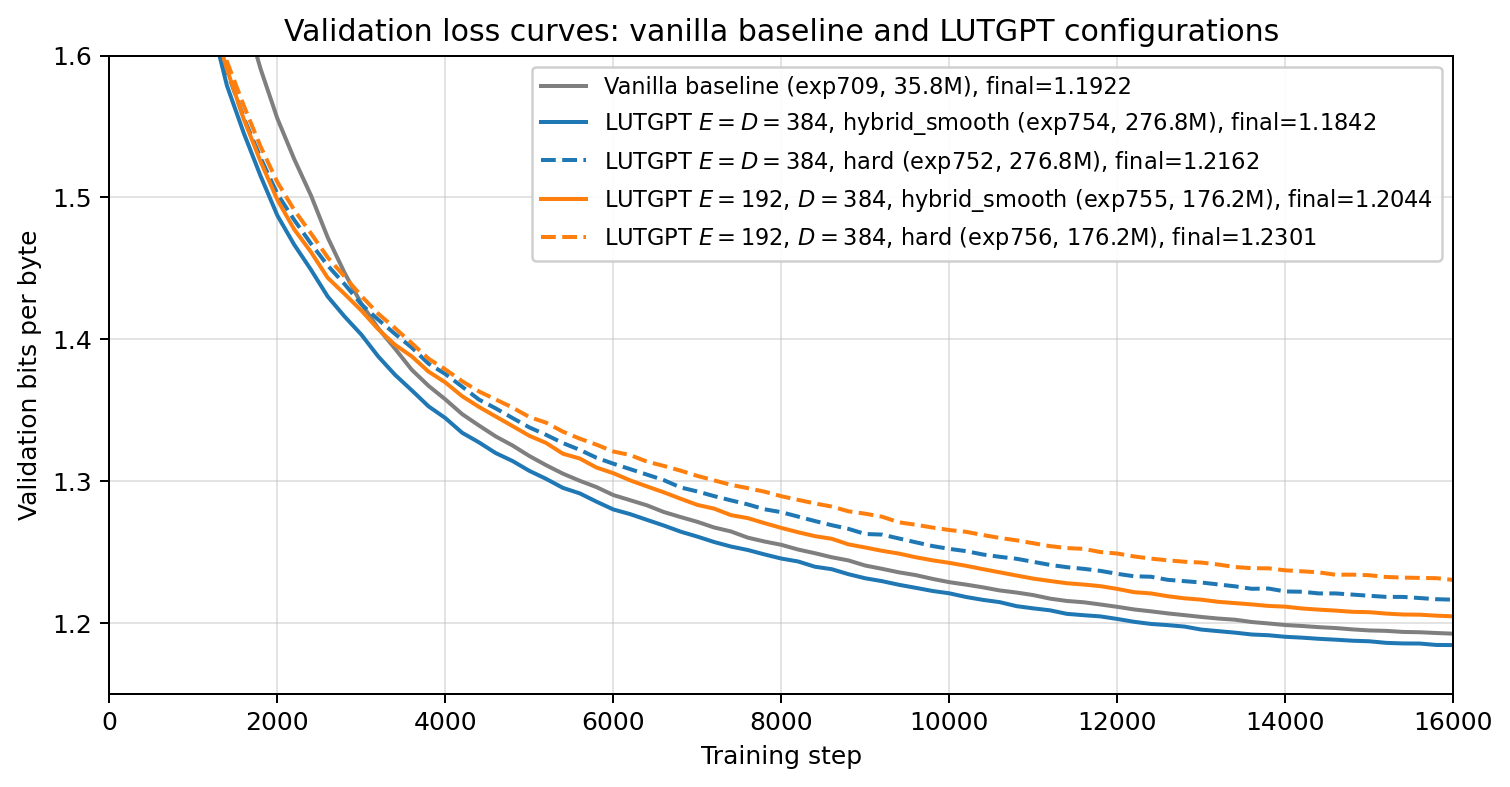
\includegraphics[width=\linewidth]{figs/val_curves.png}
\caption{Validation bits-per-byte vs.\ training step for the five runs reported in Section~\ref{sec:experiments}. Solid lines: hybrid-smooth-trained models; dashed lines: hard-trained models. Vanilla baseline (\texttt{exp709}) in grey, full-width LUTGPT pair (\texttt{exp754} hybrid-smooth, \texttt{exp752} hard) in blue, narrow-backbone LUTGPT pair (\texttt{exp755} hybrid-smooth, \texttt{exp756} hard) in orange. Eval-mode-only measurements from Section~\ref{ssec:exp-soft-hard} (the soft-trained models scored under hard forward) are not curves and appear only in the table above.}
\label{fig:val-curves}
\end{figure}

\subsection{Wall-clock-matched hard training}
\label{ssec:exp-wallclock}

\texttt{exp760} extends the narrow-backbone hard run \texttt{exp756} from $16{,}000$ to $24{,}000$ steps, keeping every other setting identical (the architecture of Section~\ref{ssec:exp-narrow}, the training recipe of Section~\ref{sec:training}, the cosine schedule re-fit over the longer horizon). The motivation is that the hard forward is roughly $1.6\times$ faster per step than the hybrid-smooth forward ($3.4$ h vs $5.4$ h at $16{,}000$ steps): the hybrid-smooth forward gathers two rows per LUT call and blends them, and its weight-gradient backward scatters to both rows, while the hard variants of each touch only one row. The input gradient is the same full-$K$ soft surrogate in either mode (Section~\ref{ssec:backward}), so the savings come from the forward and the weight-gradient, not from the input gradient. With hard's per-step advantage in hand, $1.5\times$ more hard steps fit within a comparable wall-clock budget --- the question is whether they buy back the soft-to-hard penalty of Section~\ref{ssec:exp-soft-hard}.

\begin{center}
\begin{tabular}{lcccr}
\toprule
\textbf{run} & \textbf{trained mode} & \textbf{steps} & \textbf{wall-clock} & \textbf{val\_bpb} \\
\midrule
\texttt{exp755} & \texttt{hybrid\_smooth} & $16{,}000$ & $5.4$ h & $1.2044$ \\
\texttt{exp756} & \texttt{hard}           & $16{,}000$ & $3.4$ h & $1.2301$ \\
\texttt{exp760} & \texttt{hard}           & $24{,}000$ & $5.1$ h & $\mathbf{1.2048}$ \\
\bottomrule
\end{tabular}
\end{center}

\texttt{exp760} reaches $1.2048$ --- within $0.4$\,mb of \texttt{exp755}'s $1.2044$, i.e.\ inside eval noise --- at $5.1$ h wall-clock against \texttt{exp755}'s $5.4$ h. The $25.7$\,mb soft-to-hard gap between \texttt{exp755} and \texttt{exp756} closes entirely when the hard-trained model gets the extra $50\%$ of training steps, at no extra wall-clock cost.

\begin{figure}[!ht]
\centering
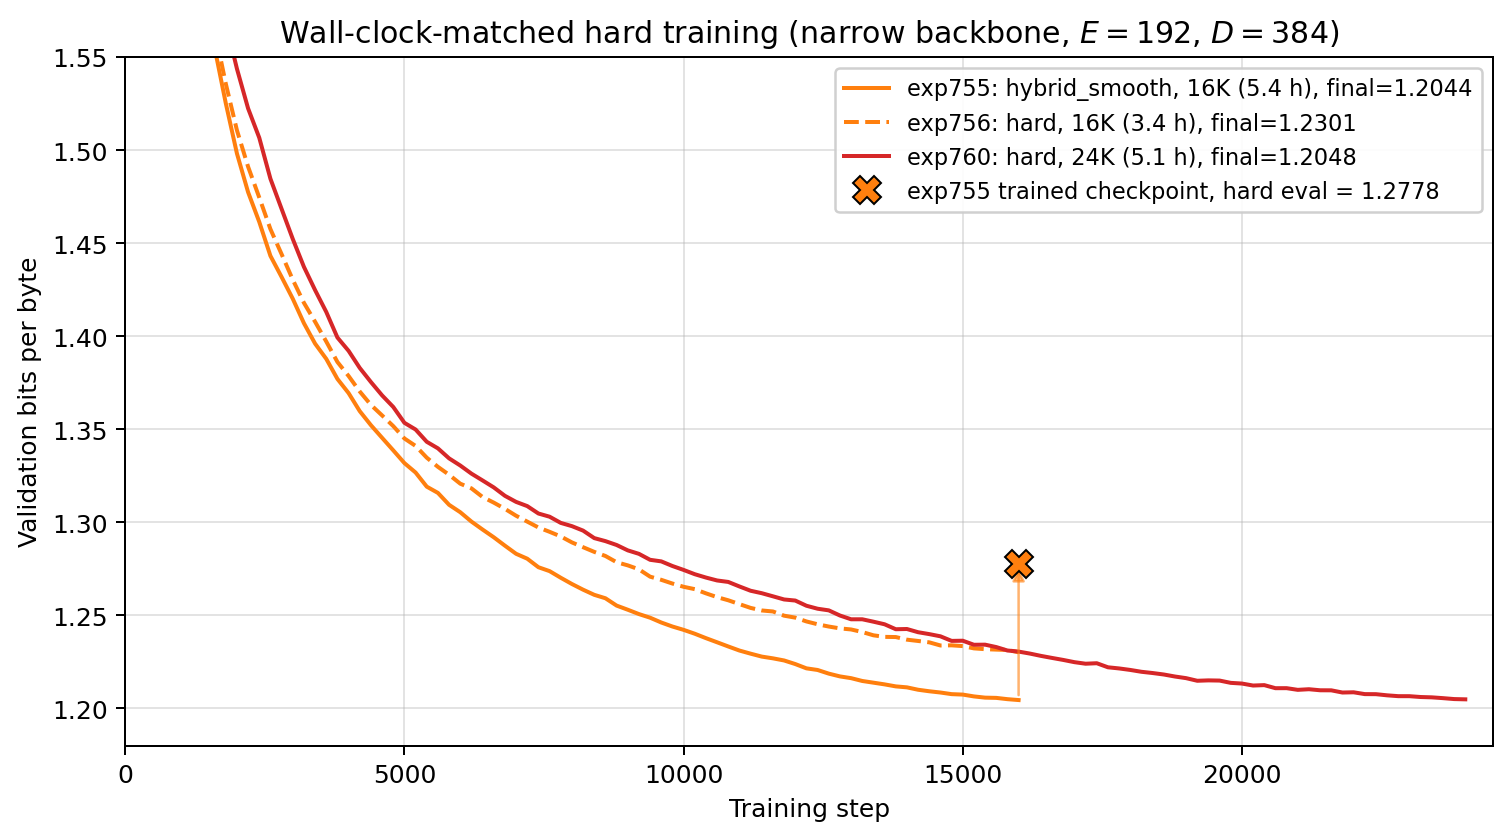
\includegraphics[width=\linewidth]{figs/val_curves_wallclock.png}
\caption{Wall-clock-matched hard training, narrow backbone ($E = 192$, $D = 384$, $176.2$\,M params). The $24$K hard-trained \texttt{exp760} (red) reaches the same val\_bpb as the $16$K hybrid-smooth-trained \texttt{exp755} (orange solid) within noise ($1.2048$ vs.\ $1.2044$) at comparable wall-clock cost ($5.1$\,h vs.\ $5.4$\,h), and ships in hard mode --- avoiding the $+73.4$\,mb soft-to-hard eval bump (orange X) that \texttt{exp755}'s trained checkpoint pays when evaluated under hard forward. Note that the other four experiments in Section~\ref{sec:experiments} are matched on \emph{training tokens}: every run sees the same $16{,}000 \cdot 24{,}576 \approx 3.93 \cdot 10^8$ tokens. \texttt{exp760} is the only run that deliberately breaks token-matching --- it matches \texttt{exp755}'s wall-clock budget instead. Hard steps are cheaper than soft steps, so $1.5\times$ as many of them fit in the same wall-clock window; \texttt{exp760} asks whether spending the budget that way closes the soft-to-hard deployment gap. The token-matched hard counterpart to \texttt{exp755} is \texttt{exp756} (orange dashed).}
\label{fig:val-curves-wallclock}
\end{figure}

\FloatBarrier

\subsection{Halving the table count}
\label{ssec:exp-tph-halved}

\texttt{exp764} applies the same wall-clock-reinvestment idea as Section~\ref{ssec:exp-wallclock} at a different knob: the number of tables per head, $\mathrm{tph}$ (Section~\ref{ssec:lutgpt-hyperparams}). Starting from \texttt{exp760}, all five LUT call sites have their $\mathrm{tph}$ halved (\texttt{qk\_lut} $256 \to 128$, \texttt{v\_lut} $256 \to 128$, \texttt{out\_proj} $512 \to 256$, \texttt{residual\_lut} $256 \to 128$, \texttt{emb\_resid\_lut} $256 \to 128$); per-LUT NAP, the dual-stream widths $E$ and $D$, and the recipe of Section~\ref{sec:training} are unchanged. The model drops from $176.2$\,M to $97.5$\,M parameters, the per-LUT HBM bandwidth halves, and per-step wall-clock at fixed effective batch falls by about $45\%$. The saved compute is reinvested into doubling the effective batch (from $24{,}576$ to $49{,}152$ tokens per step) at the same $24{,}000$ steps --- so \texttt{exp764} sees $2\times$ the training tokens of \texttt{exp760} at roughly matched wall-clock.

\begin{center}
\begin{tabular}{lccccr}
\toprule
\textbf{run} & \textbf{params} & \textbf{tokens} & \textbf{steps} & \textbf{wall-clock} & \textbf{val\_bpb} \\
\midrule
\texttt{exp760} & $176.2$\,M & $5.90 \cdot 10^{8}$ & $24{,}000$ & $5.1$ h & $\mathbf{1.2048}$ \\
\texttt{exp764} & $97.5$\,M  & $1.18 \cdot 10^{9}$ & $24{,}000$ & $5.7$ h & $1.2116$ \\
\bottomrule
\end{tabular}
\end{center}

\texttt{exp764} reaches $1.2116$ --- $6.8$\,mb above \texttt{exp760} at $55\%$ of its parameter count, half its per-LUT HBM bandwidth, and comparable wall-clock. The trade-off curve along the $\mathrm{tph}$ axis is gentle in this neighborhood: halving the table count and reinvesting the saved compute into twice as many training tokens leaves the loss almost where it was. The cheaper-to-store, cheaper-to-fetch model is the natural choice when deployment HBM and bandwidth budgets dominate.

\begin{figure}[!ht]
\centering
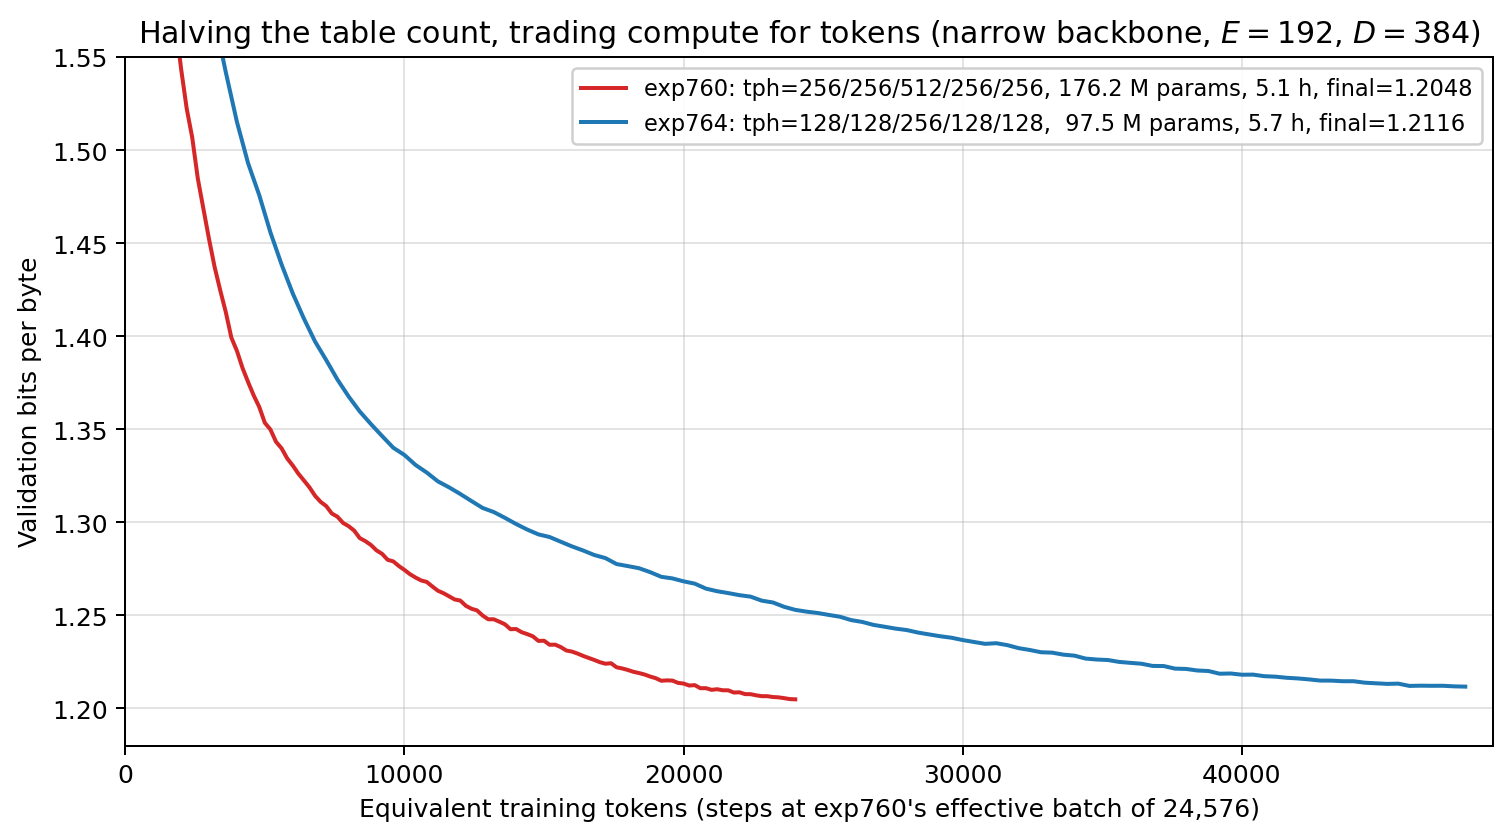
\includegraphics[width=\linewidth]{figs/val_curves_tph_halved.png}
\caption{Halving the table count, narrow backbone ($E = 192$, $D = 384$). The x-axis is normalised to \texttt{exp760}'s effective batch ($24{,}576$ tokens per step), so \texttt{exp764}'s $24{,}000$ steps at twice that batch plot as $48{,}000$ ``equivalent steps'' --- the two curves are then directly comparable at matched training tokens. At every matched-token point along the curve, \texttt{exp764} (blue, $97.5$\,M params, half the per-LUT HBM bandwidth) sits a few mb above \texttt{exp760} (red, $176.2$\,M params); spending twice the tokens recovers most of the per-token gap that the smaller tables open up, and the final $1.2116$ is only $6.8$\,mb above \texttt{exp760}'s $1.2048$ at comparable wall-clock ($5.7$\,h vs.\ $5.1$\,h).}
\label{fig:val-curves-tph-halved}
\end{figure}

\FloatBarrier

\subsection{Summary}
\label{ssec:exp-summary}

The six training runs reported in Sections \ref{ssec:exp-baseline}--\ref{ssec:exp-tph-halved} sketch the loss picture at this scale on a single set of axes:

\begin{itemize}[leftmargin=*,topsep=2pt,itemsep=1pt]
\item Untied vanilla \texttt{MinimalGPT+RoPE} (\texttt{exp709}) at $35.79$\,M params lands at $1.1922$. This is the anchor.
\item LUTGPT at full backbone width (\texttt{exp754}, $E = D = 384$, $276.8$\,M params, hybrid-smooth) reaches $1.1842$ --- $8.0$\,mb below the vanilla baseline at $7.7\times$ the parameter count. The LUT family is on vanilla's side of the curve at matched data and matched training-token budget.
\item LUTGPT at narrow backbone width (\texttt{exp755}, $E = 192$, $D = 384$, $176.2$\,M params, hybrid-smooth) reaches $1.2044$ --- $12.2$\,mb above the vanilla baseline at $4.9\times$ the parameter count. The rank-coded backbone where the LUTs compute can be halved without significantly hurting loss.
\item The naive ``train soft, ship hard'' pipeline pays a $65$--$73$\,mb eval bump (Section~\ref{ssec:exp-soft-hard}). Training natively in hard mode for the same number of steps closes $30$--$50$\,mb of that gap (\texttt{exp752}, \texttt{exp756}); spending the soft-mode wall-clock budget on additional hard-mode steps closes the rest. The narrow-backbone wall-clock-matched comparison \texttt{exp760} ($24$K hard, $5.1$ h) reaches $1.2048$, matching \texttt{exp755}'s $1.2044$ within noise --- and ships in hard mode by construction.
\item Halving the table count $\mathrm{tph}$ at every LUT call site (Section~\ref{ssec:exp-tph-halved}) shrinks the model from $176.2$\,M to $97.5$\,M parameters and halves the per-LUT HBM bandwidth. The saved per-step compute is reinvested into doubling the training-token budget at the same step count; the resulting \texttt{exp764} reaches $1.2116$, only $6.8$\,mb above \texttt{exp760} at comparable wall-clock. The $\mathrm{tph}$ axis is a cheap one to trade against when the deployment target is bandwidth-bound rather than loss-bound.
\end{itemize}

\FloatBarrier

% =========================================================================
\section{Open problems}
\label{sec:open}

Two residual matmul interfaces remain in LUTGPT, and both are open research problems whose resolution would close the loop to end-to-end LUT-class hardware execution.

\paragraph{LUT-based attention.} \texttt{softmax}$(Q \cdot K^\top) \cdot V$ is the one operation in the backbone that we did not replace with a LUT-class primitive. The difficulty is reproducing softmax's data-dependent resolution --- focusing sharply on a few keys when the match is confident, spreading broadly when it is uncertain --- inside a rank-coded primitive. Pure sign-pack lookups cannot produce a continuous attention distribution; the LUT family would need an additional mechanism (a learnt mixing kernel, a sparse top-$k$ readout, or something else) for this. We do not solve this here.

\paragraph{LUT-based unembedder.} The linear layer $\R^D \to \R^{|V|}$ producing logits is the second matmul interface. The difficulty is generating magnitude-coded logits over a 32{,}768-way vocabulary from a rank-coded representation, in a way that preserves the gradient signal a cross-entropy loss expects. We have no candidate replacement that we are confident about; the D-stream architecture exists precisely because the unembedder needs Euclidean input.

Resolving either problem would close the gap independently of the other; resolving both would make LUTGPT end-to-end LUT-class, and the hardware story above becomes a complete description of the model rather than a description of its backbone.

% =========================================================================
\section{Conclusion}

We have presented LUTGPT, a transformer-class model in which every attention projection and every residual contribution is a differentiable lookup table, with a soft-surrogate backward, two forward modes, and a published architecture that matches a vanilla, RoPE-augmented baseline with a separate unembedder on the nanochat data, with the comparison hyperparameters matched on both sides. On current GPU hardware LUTGPT is not competitive in wall-clock; on the abstract level of backbone bandwidth-per-token and active-parameter-per-token it shows a $\sim$20$\times$ higher compression density than the matched baseline. We have been explicit about which matmul interfaces remain --- SDPA and the linear unembedder --- and treat both as open problems. The contribution of this report is two-fold: the architectural existence proof that the rank-coded LUT family extends to a real text-data model at meaningful scale, and the explicit identification of the architectural properties that would make this family the preferred choice on specialised rank-coded sparse-lookup hardware.

% =========================================================================
\section*{Acknowledgements}

We thank Yuval Aviel for several useful discussions during the development of this work, and the Nebius group for providing the GPU compute on which the experiments in Section~\ref{sec:experiments} were run.

% =========================================================================
\appendix
\section{Implementation notes}
\label{sec:engineering}

The code accompanying this report is the \texttt{spiky} repository at \url{https://github.com/anatoli-starostin/spiky}, on the \texttt{publish/lutgpt} branch. The LUT primitive of Section~\ref{sec:primitive} lives in \texttt{src/spiky/lutorch/fast\_multi\_head\_lut.py} as \texttt{FastMultiHeadLut}.

Two end-to-end entry points reproduce the report's models at different scales:

\begin{itemize}[leftmargin=*,topsep=2pt,itemsep=2pt]
\item \texttt{examples/lutgpt/} ships the narrow-backbone reference configuration of Section~\ref{ssec:exp-narrow} ($E = 192$, $D = 384$, hybrid-smooth forward for $16{,}000$ steps; the published \texttt{exp755} recipe). \texttt{train.py} reads \texttt{config.json} and builds the model of Section~\ref{ssec:lutgpt-arch}. Requires a local checkout of \texttt{nanochat}~\citep{karpathy_nanochat} pointed to by the \texttt{NANOCHAT\_ROOT} environment variable for the tokeniser, dataloader, and bpb evaluator.
\item The single-GPU walkthrough \texttt{workbooks/nanochat\_walkthrough.ipynb} loads the tokenised dataset, trains the vanilla \texttt{MinimalGPT+RoPE} baseline of Section~\ref{ssec:baseline}, then trains a LUTGPT at the full-width architecture of Section~\ref{ssec:exp-headline} (\texttt{exp754}; $E = D = 384$, $d_v = 64$) at a reduced budget (device batch $8$, $8{,}000$ steps) so the whole run fits in a few hours.
\end{itemize}

% =========================================================================
\begin{thebibliography}{99}

\bibitem[Izhikevich(2025)]{manifesto}
E. Izhikevich.
\newblock The spiking manifesto: ranking-coded computation and differentiable lookup tables.
\newblock Technical report, 2025. [internal reference; placeholder citation]

\bibitem[Karpathy(2025)]{karpathy_nanochat}
A. Karpathy.
\newblock nanochat.
\newblock \url{https://github.com/karpathy/nanochat}, 2025.

\bibitem[Vaswani et al.(2017)]{vaswani2017attention}
A. Vaswani, N. Shazeer, N. Parmar, J. Uszkoreit, L. Jones, A. N. Gomez, L. Kaiser, I. Polosukhin.
\newblock Attention is all you need.
\newblock \emph{NeurIPS}, 2017.

\bibitem[Su et al.(2021)]{su2021roformer}
J. Su, Y. Lu, S. Pan, B. Wen, Y. Liu.
\newblock RoFormer: enhanced transformer with rotary position embedding.
\newblock \emph{arXiv:2104.09864}, 2021.

\bibitem[Chen et al.(2023)]{chen2023lion}
X. Chen, C. Liang, D. Huang, E. Real, K. Wang, Y. Liu, H. Pham, X. Dong, T. Luong, C.-J. Hsieh, Y. Lu, Q. V. Le.
\newblock Symbolic discovery of optimization algorithms.
\newblock \emph{NeurIPS}, 2023.

\bibitem[Loshchilov \& Hutter(2017)]{loshchilov2017decoupled}
I. Loshchilov, F. Hutter.
\newblock Decoupled weight decay regularization.
\newblock \emph{ICLR}, 2017.

\end{thebibliography}

\end{document}
